%!TEX program = xelatex
%windows、macOS用户都可用
\documentclass[UTF8, punct, oneside,fontset=none]{ctexbook}
\usepackage[windows]{nsfc}
%macOS用户独享
%\documentclass[UTF8, punct, oneside]{ctexbook}
%\usepackage[macos]{nsfc}
%用来对比模版有无变化。对比时,请注释掉以下语句:
%\renewcommand{\input}[1]{\vspace{\baselineskip}}
%如果你个人文件和文件夹以⚠︎开头进行命名,可以省心更新模版。参见README.md

\pagestyle{empty} % 第二页以后页码空白
\usepackage[a4paper, left = 3.2cm, right = 3.2cm, top = 2.72cm, bottom = 2.54cm]{geometry}%页边距

\usepackage{times}

\usepackage{setspace}

\usepackage{comment}

\graphicspath{{figures/}}   % 设置图片所存放的目录
\begin{document}
%\thispagestyle{empty}    % 首页页码空白

{\centering\zhkai\fontsize{16pt}{21pt}\selectfont
\setlength{\baselineskip}{21pt}%最后设置,防止被fontsize中的覆盖
\hspace{30pt}\textbf{报告正文}\par
\vspace{5.46pt}}%0.2(行距倍数)*21(行距)*1.3(word)

%\begin{comment}
{\zhkai\fontsize{14pt}{22pt}\selectfont
 \setlength{\baselineskip}{22pt}%最后设置,防止被fontsize中的覆盖
参照以下提纲撰写,要求内容翔实、清晰,层次分明,标题突出。
\textbf{\color{YSFblue}请勿删除或改动下述提纲标题及括号中的文字。}\par
\vspace{.3pt}}%0.5(行距倍数)*22(行距)*1.3(word)
%\end{comment}

\chapter{\textbf{立项依据与研究内容}(建议8000字以下):}
\vspace{3pt}
\section{\textbf{项目的立项依据}\kg{0.2em}(研究意义、国内外研究现状及发展动态分析,需结合科学研究发展趋势来论述科学意义;或结合国民经济和社会发展中迫切需要解决的关键科技问题来论述其应用前景。附主要参考文献目录);}

%\excludecomment{MS}%用来对比模版有无变化
%或者下边这种方法
%\renewcommand{\input}[1]{ }%用来对比模版有无变化

\begin{MS}
	
\subsection{研究意义}
波动方程是二阶双曲型偏微分方程\cite{bedford1994},可用于描述地震波、水波、电磁波等自然界中的波动现象,广泛的应用于无损检测、地震预测、生物医学成像等各个工程领域。
发展波动方程的高精度分析方法将有助于提升如无损检测准确率、医学成像精度等。
由于实际工程问题中通常涉及复杂几何区域、材料非均质等一系列问题,采用理论分析手段研究波动问题难以获得解析解。于是,数值仿真分析成为了研究波动方程的重要工具。
在波动问题的主流数值分析方法中,时间域和空间域将独立离散为有限个分布节点用于近似位移变量,其中空间域通常采用基于变分原理的弱形式进行离散分析,如有限元法等。
在变分原理的帮助下,基于弱形式型的方法具有求解精度高、稳定性强的特点,适用于复杂空间几何构型。
而时间域则采用基于微分方程的强形式进行离散分析,如有限差分法等。
该类方法通常采用迭代形式进行程序实现,实现过程简单高效。
但基于强形式型的方法在计算精度和稳定性方面均低于基于弱形式型的方法,计算误差将随着迭代步的增加而累积增大。

波动方程数值分析的另一种思路是将时间域作为第四维空间进行混合离散,并采用基于哈密顿变分原理的弱形式进行求解。
该类方法将提升整体的求解精度,有利于时空区域自适应节点加密过程。
求解过程无需进行迭代,可采用整体并行计算求解提高效率。
然而自上世纪九十年代Hughes首次采用时空混合离散结合间断伽辽金法求解波动问题\cite{hughes1988}以来,该类方法发展缓慢。
\textbf{
主要的原因是该方法在求解稳定的前提下并不能适用于任意节点分布情况,导致其未能广泛应用于复杂的实际工程问题中,阻碍了时空混合离散伽辽金法的发展。
}
造成时空混合离散伽辽金法无法适用任意节点分布情况的原因主要有三点:

首先是\textbf{时域末端虚位移本质边界条件的施加问题}。
波动方程的时空混合离散伽辽金法通过哈密顿变分原理建立相对应的弱形式,
如图 \ref{fg:hamilton} 所示,哈密顿原理要求虚位移$\delta q$在初始时刻$t_0$和末端时刻$t_1$为零,即$\delta q(t_0)=\delta q(t_1)=0$,以等价于欧拉--拉格朗日方程\cite{arnold1978}。
在传统边值问题中,虚位移本质边界条件通常伴随着位移本质边界条件。
当采用伽辽金法进行求解时,即虚位移和位移采用相同的离散方式,位移及其虚位移涉及本质边界条件的自由度数量相同。
采用矩阵压缩技术直接施加本质边界条件时,可保持刚度矩阵为方阵且可逆。
然而,波动方程在时间维度上属于初值问题,即已知初始时刻位移和速度,$q(t_0)=q_0,\dot q(t_0) = \dot q_0$,时域末端边界条件未知。
如图 \ref{fg:direct} 所示,直接施加初始时刻位移边界条件将填补末端时刻虚位移为零造成刚度矩阵却是的部分。
而初始时刻虚位移不再要求为零,初始时刻速度边界条件可在此处作为自然边界条件施加。
但该方法可实施的前提是\textbf{涉及初始时刻和末端时刻的自由度数量需要保持一致,并不适用于任意节点分布情况。}
间断伽辽金法则是在弱形式中增加了哈密顿原理时域边界条件相关项,以规避虚位移本质边界条件的施加。
但是,该方法需要在时域上采用如图 \ref{fg:slab} 所示的分块离散以保证整体A--稳定性条件\cite{hughes1988}。
\textbf{时域分块网格不仅限制了节点布置,而且在时域块状边界处采用非连续的位移进行近似,增加了由位移自由度数量,提高了计算的复杂度和耗时。}


\begin{figure}[!h]
    \centering 
    \includegraphics[width=\textwidth]{figures/Hamilton.png}
    \caption{哈密顿原理与欧拉--拉格朗日方程等价性}
    \label{fg:hamilton}
\end{figure}

\begin{figure}[!h]
    \centering 
    \includegraphics[width=0.8\textwidth]{figures/stiffness.png}
    \caption{直接施加时域末端虚位移本质边界条件}
    \label{fg:direct}
\end{figure}

\begin{figure}[!h]
    \centering 
    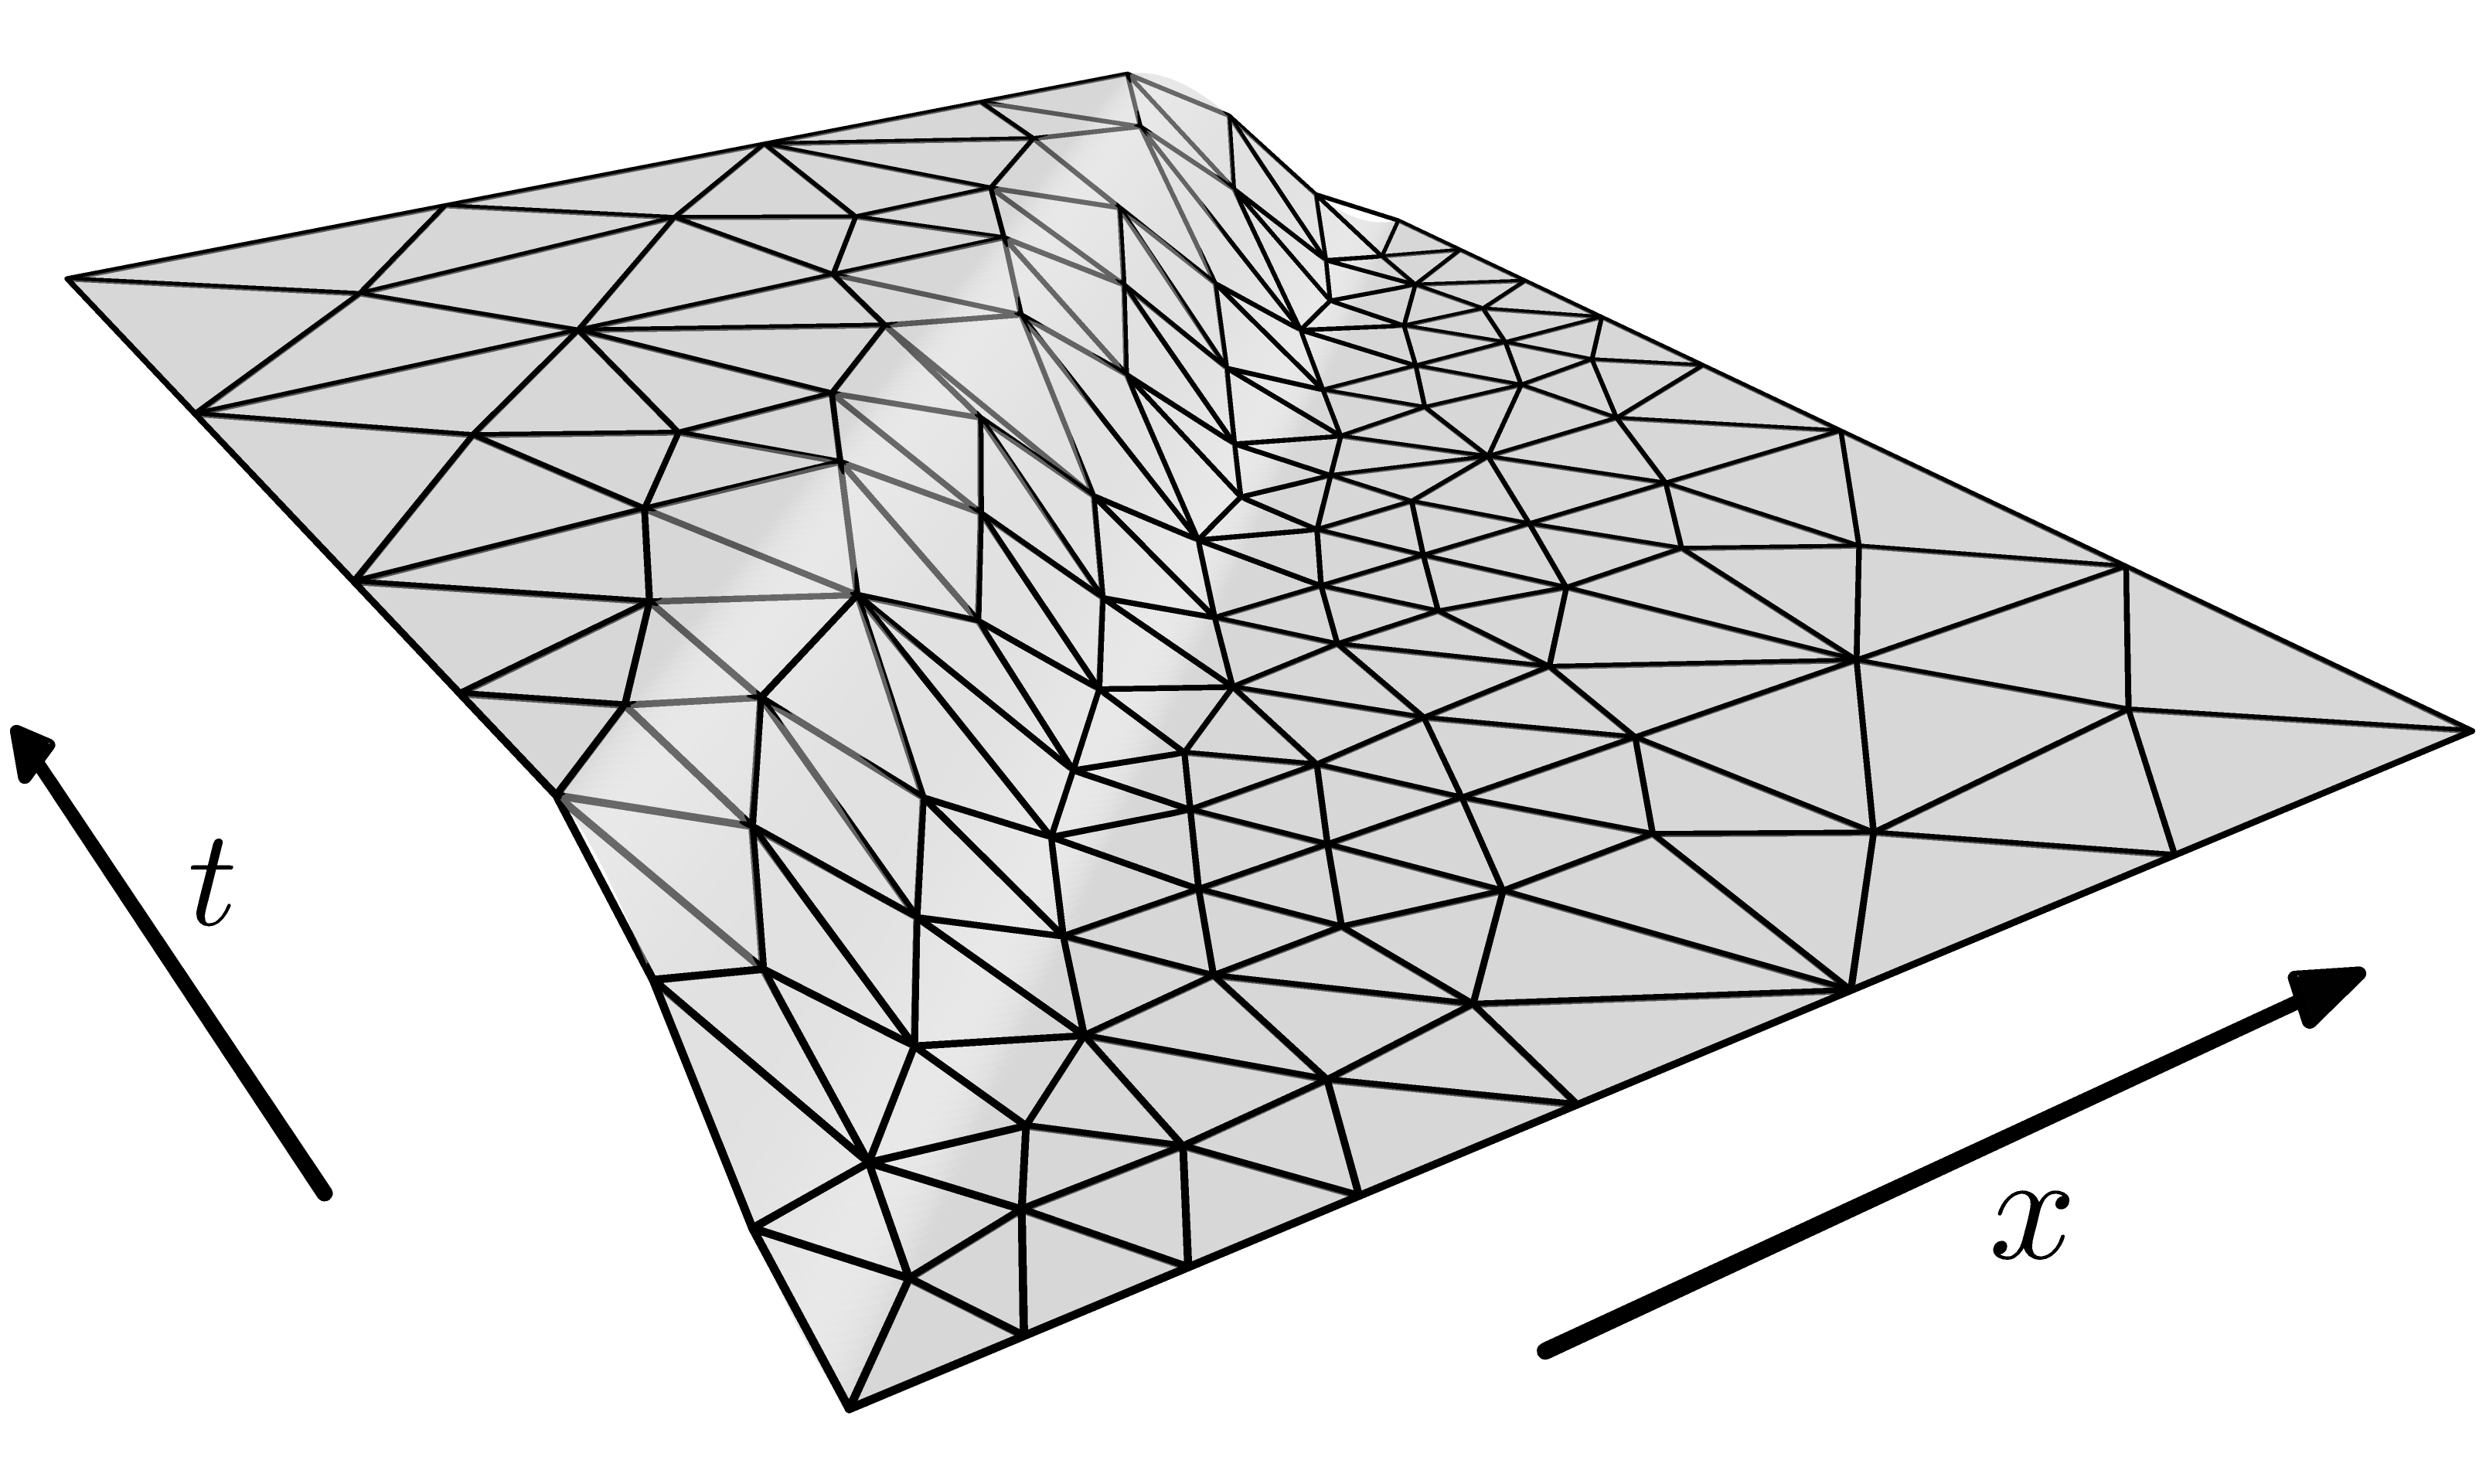
\includegraphics[width=0.8\textwidth]{figures/wave.png}
    \caption{时空混合离散间断伽辽金法}
    \label{fg:slab}
\end{figure}

% \begin{equation*}
% \begin{split}
% 	\delta \Phi&=\int_{t_0}^{t_1} \delta q \frac{\partial L}{\partial q} + \delta \dot q \frac{\partial L}{\partial \dot q} dt\\ &=\int_{t_0}^{t_1} \delta q({\color{blue}\frac{\partial L}{\partial q} - \frac{\partial}{\partial t}\frac{\partial L}{\partial \dot q}}) dt + {\color{red}\delta q \left . \frac{\partial L}{\partial \dot q}\right \vert_{t_0}^{t_1}}\\&= 0
% \end{split}
% \xrightarrow{{\color{red}\delta q(t_0)=\delta q(t_1)=0}}
% \color{blue}\left \{\begin{split}&\frac{\partial L}{\partial q} - \frac{\partial}{\partial t}\frac{\partial L}{\partial \dot q}=0\\& q(t_0) = q_0,\;\dot q(t_0) = \dot q_0\end{split}\right .
% \end{equation*}

其次是\textbf{数值色散问题}。
数值色散问题是由于离散控制方程的局部截断误差过大,导致不同频率波的波速不一致引起的数值振荡现象。
抑制数值色散现象主要通过以下方法:
\textcircled{\textbf{\small 1}}
调整时间域与空间域节点离散间距,以满足Courant–-Friedrichs-–Lewy(CFL)条件或谱半径稳定性条件,提高近似分辨率。
该方法需要限制节点间距比例,不适用于任意节点分布情况。
\textcircled{\textbf{\small 2}}
引入人工耗散项缓解高频振动,该方法通常需要引入强形式作为稳定人工耗散项,强形式中包含变量的高阶导数,不适合线性近似方案。
且人工耗散项可能会引起数值耗散问题,降低计算精度。
\textcircled{\textbf{\small 3}}
提高时域离散阶次,以降低局部截断误差,缓解振动现象。
该方法相较于前两种方法更为直接有效,且适用于任意节点分布情况。
然而,\textbf{构造高阶形函数对于基于单元拓扑信息近似的有限元法来说并非易事,特别是对于高维时空域混合离散情况。}
不同于传统有限元法,无网格法\cite{Zhang2004a}是一类仅依据节点位置信息构建高阶光滑形函数的近似方法,近年来得到了快速地发展和广泛地应用。
在众多无网格近似方案中,再生核无网格近似可构造满足任意阶次一致性条件的无网格形函数。
\textbf{在任意节点分布下,再生核无网格近似可通过分别调整时间域和空间域的近似阶次,以降低局部截断误差,缓解数值色散引起的振荡现象。}

最后是\textbf{高维度网格划分问题}。
相较于时间域和空间域单独离散的情况,时空混合离散需要采用高一维度近似方案进行分析。
传统有限元法通常在复杂几何区域网格化分困难,尤其是高维及高阶情况,通常需要人工修正网格以保证计算结果的可靠性。
无网格法虽然在建立形函数过程中无需依赖网格,但在结合伽辽金法求解时,仍然需要网格作为背景积分域进行数值积分。
与有限元法不同的是,伽辽金无网格法无需采用无网格节点作为背景积分域顶点。
采用结构型网格作为背景积分域也适用于自适应节点加密过程。
如图所示,传统有限元法在节点加密处,网格数量也随之增加。
难以保证网格质量,影响求解精度。
而\textbf{无网格法自适应节点加密过程中背景积分域可以不需要随节点数增加而细划,降低高维背景积分域划分难度,有效缓解网格畸变引起的精度下降}。

针对上述时空混合离散伽辽金法的瓶颈问题,本项目拟研究时空混合离散伽辽金法中虚位移本质边界条件施加方案,并结合再生核近似的伽辽金无网格法缓解数值色散问题,建立高维时空混合离散自适应节点加密方案,
旨在为波动问题发展一种适应于任意节点分布的稳定伽辽金无网格分析方法,为实际工程中的波动问题提供一种精确、鲁棒和高效的数值工具。

\subsection{国内外研究现状及发展动态}

国内外诸多学者针对时空混合离散伽辽金无网格法的相关问题进行了广泛的研究,主要研究内容可分为时空混合离散方案、数值色散问题稳定方案和伽辽金无网格法求解波动问题三方面,下面将分别对这三方面的研究现状及发展动态进行介绍。

时空混合离散方案可在加权残余法的基础上,依据时间域和空间域使用强形式离散或弱形式离散进行分类。
第一类方法为时间域和空间域均采用强形式进行离散,如。
时间连续有限元\cite{vondanwitz2023}
最小二乘法\cite{epstein2024}。
该类方法在时域和空间域上均采用强形式进行求解,难以保证整体系统能量守恒和计算的稳定性。
第二类方法在时间域上采用强形式进行离散,而空间域上采用弱形式进行离散。
这类型离散不仅常用于时间和空间独立近似情况,如,也是时空
是对空间维度进行分部积分。
第三类方法在时间和空间维度上均进行分部积分,该类方法满足哈密顿变分原理。
也是最初开展
然而,基于哈密顿原理的时空混合离散方案需要要求,目前还缺乏一种施加虚位移本质边界条件的方法。

时空混合离散方案时哈密顿原理,
然而,哈密顿原理虚位移本质边界条件施加困难的问题,。
Hou和Peters在哈密顿原理的基础上\cite{hou1994}
Hughes和Hulbert\cite{hughes1988}通过引入速度变量将二阶偏微分方程转换为两个一阶偏微分方程,并采用间断伽辽金法进行求解,规避了时域末端虚位移本质边界条件问题。


\vspace{-5pt}

\begin{REF}
	\subsection*{参考文献}
	\vspace{-50pt}
	\bibliographystyle{gbt7714-2005-numerical}
	\bibliography{ref}%参考文献
\end{REF}

\newpage%自己判断是否需要

\end{MS}


\section{\textbf{项目的研究内容、研究目标,以及拟解决的关键科学问题}(此部分为重点阐述内容)\textbf{;}}

\begin{MS}
	\subsection{研究内容}
本项目将围绕波动方程中时空混合离散伽辽金法存在的问题,
研究时域末端虚位移本质边界条件施加方案,
构建可缓解数值色散问题的时空混合离散无网格近似方案,
并引入变分一致型伽辽金无网格数值积分法,
建立绝对时空混合离散伽辽金无网格分析方法。
具体的研究内容如下:

\subsubsection*{\bfseries (1)适用于任意节点分布的时域末端虚位移本质边界条件施加方案}
在波动方程哈密顿原理的基础上,分析能量泛函中时域末端虚位移本质边界条件下位移变量的求解空间。
将传统能量泛函中的虚位移作为拉格朗日乘子,设计全新拉格朗日乘子型能量泛函。
分析新建立的能量泛函中,经过拉格朗日乘子法投影后的位移变量空间与原空间的等价性。
同时在全新的能量泛函中引入应力边界条件与初始时刻动量边界条件,验证相对应拉格朗日乘子型伽辽金弱形式的变分一致性,证明其与欧拉--拉格朗日方程的等价性。


\subsubsection*{\bfseries (2)可缓解数值色散问题的时空混合离散再生核无网格近似方案}
探究拉格朗日乘子型能量泛函的稳定性条件,构建考虑时空混合离散阶次的局部截断误差估计表达式。
研究考虑时间维度的再生核无网格近似框架,以时空混合离散截断误差估计为基础,确定误差稳定时的再生核近似基向量中时间维度相关单项式。
根据确定基向量表达式,调整再生核近似中核函数影响域大小和表达式,以确保再生核近似中矩量矩阵可逆。
最后,通过数值算例验证所提无网格近似方案能否缓解数值色散问题。

\subsubsection*{\bfseries (3)时空混合离散下变分一致型伽辽金无网格数值积分方案}
根据时空混合离散无网格近似中基向量的元素,确定波动问题拉格朗日乘子型伽辽金弱形式的积分约束条件。
以再生光滑梯度理论框架为基础,构建时空混合离散下满足积分约束条件的变分一致型伽辽金无网格数值积分方法。
在四维情况下,引入四面体柱或六面体柱单元作为背景积分域。通过再生光滑梯度的一致性条件,优化全局数值积分点数量,确定积分点位置和权重。
最后,通过时空混合离散分片试验,测试所提伽辽金无网格数值积分方案的变分一致性和计算精度。

\subsubsection*{\bfseries (4)绝对时空混合离散高效伽辽金无网格分析方法}
将时空混合离散再生核无网格近似引入拉格朗日乘子型伽辽金弱形式,结合变分一致型伽辽金无网格数值积分方案,建立波动方程时空混合离散控制方程。
进一步分析离散控制方程表达式,利用离散控制方程刚度矩阵的相识性,优化程序结构,降低内存开销。
同时,基于位移解的梯度变化,制定相对应的无网格自适应节点加密方案。
在求解离散控制方程时引入成熟并行计算库,实现时间域和空间域同时并行计算,
建立绝对时空混合离散高效伽辽金无网格分析方法及其通用数值仿真程序。通过典型波动问题和实际工程算例验证所提方法的有效性和可靠性。

\subsection{研究目标}
本项目完成上述各项研究内容旨在建立绝对时空混合离散伽辽金无网格分析方法,该方法能适用于任意布置的节点离散情况,缓解数值色散问题,
提升分析波动问题时的计算效率和稳定性。具体的研究目标包括:
\begin{enumerate}[label={\rmfamily (\theenumi)},left=24pt]
    \item 建立适用于任意节点离散的时域末端虚位移本质边界条件施加方案,提升时空混合离散伽辽金法对节点离散的鲁棒性;
    \item 提出适用于波动方程再生核无网格近似方案,缓解波动问题时空混合离散伽辽金无网格法的色散问题;
    \item 设计适用于高维波动方程的变分一致型伽辽金无网格法数值积分方案,降低高维背景积分域划分难度,提升计算效率;
    \item 发展任意节点分布的稳定时空混合离散高效伽辽金无网格分析方法,为实际波动问题提供可靠、稳定的数值工具。
\end{enumerate}

\subsection{拟解决的关键科学问题}

本项目拟解决的关键科学问题如下:

\subsubsection*{\bfseries (1)如何构建与哈密顿原理等价的时域末端虚位移本质边界条件}
哈密顿原理要求时域末端虚位移等于零,才可使相对应的弱形式等价于欧拉--拉格朗日方程。
由于在实际问题中,时域末端边界条件通常是未知的。单独令时域末端虚位移为零将导致整体弱形式丧失变分一致性,计算结果将出现与实际不符的情况。
目前已有方法通常是采用间断伽辽金格式规避时域末端边界,但需要采用分块网格技术提高求解的稳定性。
因此,如何正确施加时域末端虚位移本质边界条件,使时空混合离散伽辽金法适用于任意节点离散情况,是本项目研究内容(1)的关键科学问题。

\subsubsection*{\bfseries (2)如何确定时空混合无网格近似基向量阶次对求解稳定性的影响机理}
波动方程属于二阶双曲型偏微分方程,求解过程中时域离散节点间距过大将引起数值色散问题,导致计算结果发散。
传统方法可减小离散节点间距缓解该问题,随之将伴随自由度的增加所引起的计算量增大,不适合任意节点离散情况。
增加稳定项也可提升计算的稳定性,但节点间距过小时该方法将出现数值耗散问题,也不适用于任意节点离散情况。
本项目的研究内容(2)旨在利用无网格构造高阶再生特性形函数的便利性,缓解数值色散问题。因此,确定时空混合离散无网格近似基向量阶次对求解稳定性的影响机理,是该研究内容的关键科学问题。

\subsubsection*{\bfseries (3)如何优化时空混合离散变分一致伽辽金无网格数值积分方案}
由于无网格形函数通常为有理式,伽辽金无网格法需要采用变分一致型数值积分方案以保证计算精度。
变分一致型数值积分方案可通过形函数导数的一致性条件,优化全局数值积分点个数。
最终的数值积分点个数将直接影响时空混合离散伽辽金无网格法的计算效率。
相较于传统时间域与空间域分别离散的方法,时空混合离散将增加时间维度的离散,离散维度比传统方式增加了一个维度。
采用变分一致型伽辽金无网格数值积分方案时,需要额外考虑与时间维度相关的单项式积分约束条件与一致性条件。然而,为了缓解数值色散问题,时间维度相关的单项式阶次将不同于空间维度相关的单项式阶次。
如何在时空混合离散情况下优化变分一致型伽辽金无网格数值积分方案,提升整体计算效率,是本项目研究内容(3)的关键科学问题。


\end{MS}

\section{\textbf{拟采取的研究方案及可行性分析}(包括研究方法、技术路线、实验手段、关键技术等说明);}

\begin{MS}
	%公式的上下间距
\setlength{\abovedisplayskip}{0pt}
\setlength{\belowdisplayskip}{0pt}

\subsection{研究方法与技术路线}

本项目将采用理论推导结合数值验证的方法进行研究,
首先,理论推导哈密顿原理伽辽金弱形式中拉格朗日乘子型虚位移本质边界条件施加方案,并分析相对应的弱形式与欧拉--拉格朗日方程之间的等价性。
其次,基于再生核无网格近似,采用理论推导分析离散控制方程局部截断误差,并通过数值测试确定求解稳定时再生核无网格近似阶次。
随后,依托再生光滑梯度理论框架,构建适用于时空混合离散的变分一致型伽辽金无网格数值积分方案。
最后,建立适用于任意节点分布的稳定时空混合离散伽辽金无网格法,并数值验证所提方法的有效性。
具体的技术路线图如图 \ref{fg:roadmap} 所示。

\begin{figure}[!h]
    \centering 
    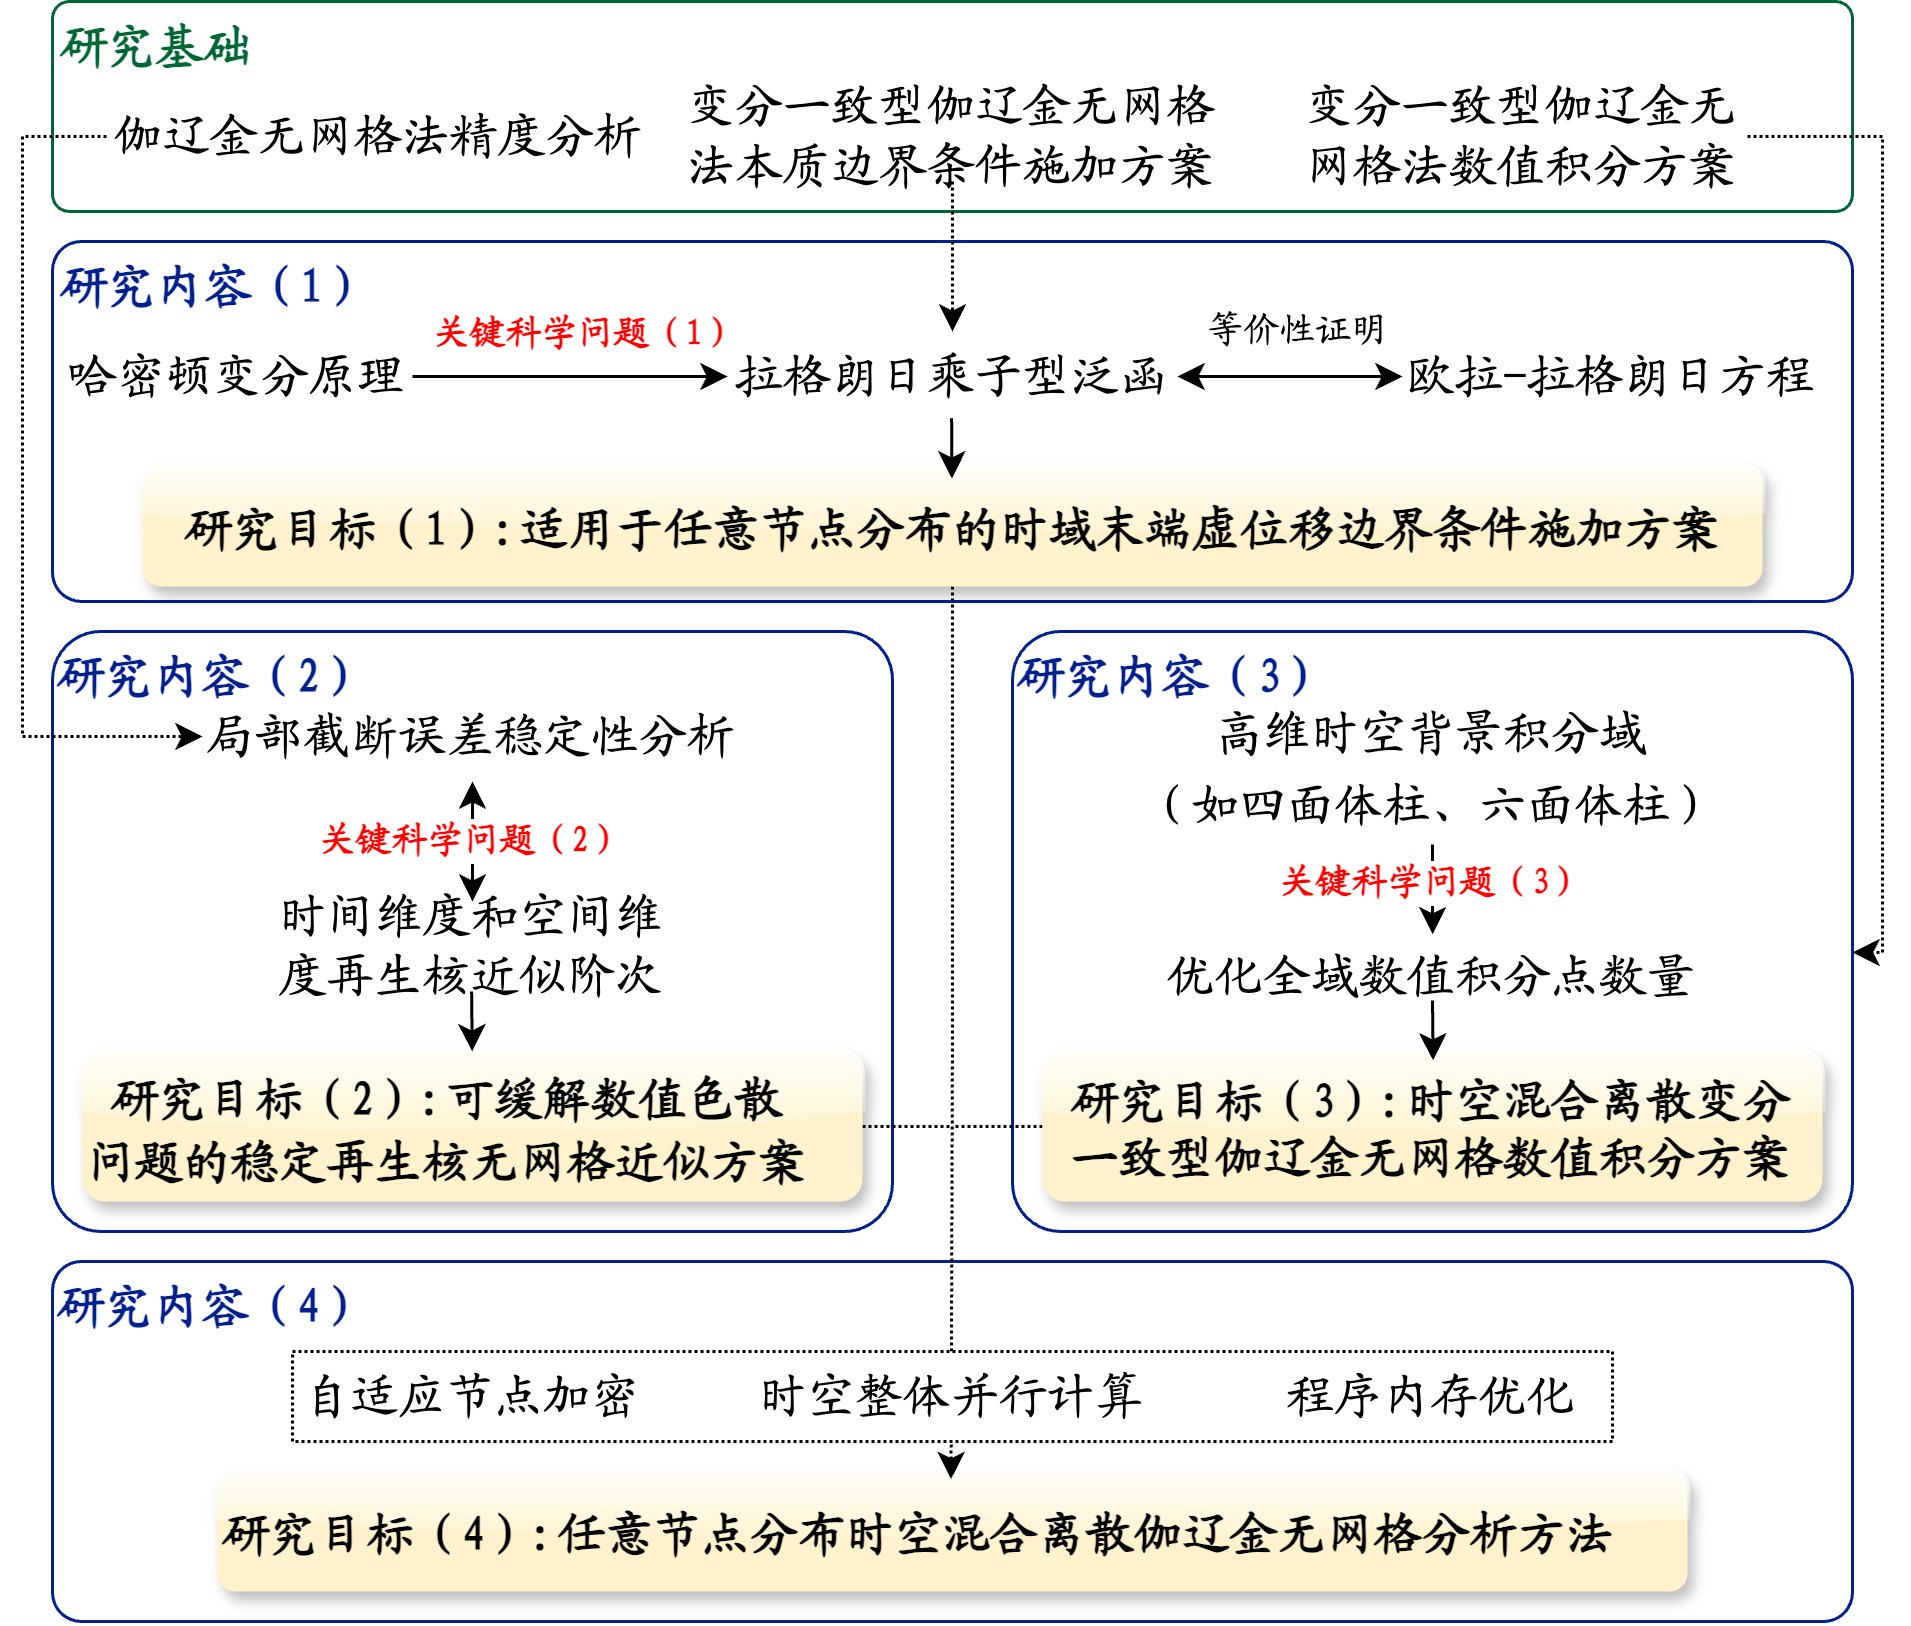
\includegraphics[width=\textwidth]{figures/roadmap.png}
    \caption{技术路线图}
    \label{fg:roadmap}
\end{figure}

\subsection{研究方案}

\subsubsection*{\bfseries (1)适用于任意节点分布的时域末端虚位移本质边界条件施加方案}
首先,查阅基于哈密顿变分原理时空混合离散有限元法的相关文献,确定虚位移本质边界条件的几种可能性。
将不同虚位移边界的方法进行数值实现,对比计算结果的稳定性和精度。
确定稳定性最优情况下的虚位移空间$\tilde V_h$,相对应的变分问题为:
\begin{equation}
    \text{find} \; u_h \in V_h, \quad a(u_h, \delta u_h) = f(\delta u_h), \quad \forall \delta u_h \in \tilde V_h
    \label{eq:1}
\end{equation}
其中,$V_h$为位移空间,$a:V\times V \rightarrow \mathbb R$为双线性算子,$f:V\rightarrow \mathbb R$为线性算子。

随后,将式\eqref{eq:1}中的虚位移$\delta u_h$作为拉格朗日乘子,设计全新拉格朗日乘子型能量泛函:
\begin{equation}
    \text{find} \; u_h \in V_h,\; p_h \in \tilde V_h, \quad
    \left \{
    \begin{split} 
        -a(u_h, \delta u_h) + a(p_h, \delta u_h) = 0,\quad &\forall \delta u_h \in V_h \\
        a(u_h, \delta p_h) = f(\delta p_h),\quad &\forall \delta p_h \in \tilde V_h
    \end{split}
    \right .
    \label{eq:2}
\end{equation}
从上式可以看出,原本式\eqref{eq:1}中的变分问题作为约束条件施加在拉格朗日乘子型伽辽金问题的弱形式中,需进一步在验证两者之间的等价性。
当等价性成立,仅需要采用常规方法对$p_h$施加本质边界条件,即可实现式\eqref{eq:1}中施加虚位移本质边界条件的效果。
同时,引入分部积分公式对式\eqref{eq:2}进行推导,通过修正$u_h$和$p_h$的边界条件,使所提的拉格朗日乘子型伽辽金弱形式满足变分一致性,并证明其与欧拉--拉格朗日方程等价。

最后,采用均布的有限元离散从数值上与传统方法进行对比,验证其计算精度。并用分均布节点离散验证所提方法求解的稳定性。

\subsubsection*{\bfseries (2)可缓解数值色散问题的稳定再生核无网格近似方案}
首先,借鉴von Neumann稳定性分析方法,在拉格朗日型能量泛函所对应的离散控制方程中引入特征解的傅立叶展开式。
同时引入无网格形函数一致性条件,推导均布节点离散下离散控制方程中通用行的局部截断误差估计$\epsilon$,
$\epsilon$应包含时间域节点间距$\Delta t$和空间域节点间距$\Delta x$相关的余项:
\begin{equation}
    \epsilon = O(\Delta t^{n_t}) + O(\Delta x^{n_x})
\end{equation}
其中,$n_t$和$n_x$分别为时间域和空间域的离散阶次。根据截断误差估计,确定空间域离散阶次为$n_x$时,消除数值色散影响所需的时间域离散阶次$n_t$。

随后,在再生核无网格近似的理论框架下,构造相对应阶次的无网格近似基向量$\boldsymbol p^{[n_x,n_t]}$:
\begin{equation}
    \boldsymbol p^{[n_x,n_t]}(x,t) = \left \{1, x, t, x^2, xt, t^2, \dots, x^{n_x}, x^{n_x-1}t, \dots, t^{n_t} \right \}^T
\end{equation}
并根据无网格形函数中矩量矩阵的可逆性,确定核函数影响域在时间维度和空间维度包含节点的个数。

% \begin{figure}[H]
%     \centering
    
% \end{figure}

最后,通过数值验证所提混合离散再生核无网格近似的一致性条件。并代入所提拉格朗日型能量泛函,通过时间域、空间域不同比例节点间距和非均布节点离散测试其是否缓解数值色散问题。

\subsubsection*{\bfseries (3)时空混合离散下变分一致型伽辽金无网格数值积分方案}
首先,根据时空混合离散无网格近似中基向量的元素,推导拉格朗日型伽辽金弱形式的积分约束条件。
引入申请人所提出的再生光滑梯度理论框架,构建满足满足积分约束条件无网格形函数再生光滑梯度,以形函数的一阶时间光滑导数为例,其表达式为:
\begin{equation}
    \tilde \Psi_{I,t}(\boldsymbol x) = \boldsymbol p^{[n_x,n_t - 1]}(\boldsymbol x) \boldsymbol G^{ - 1} \boldsymbol g_{tI}
\end{equation}
其中,$\boldsymbol G$为矩量矩阵,$\boldsymbol g_{tI}$为积分约束条件。再生光滑梯度能自动满足变分一致性条件,适用于相对应阶次的高斯积分方案。

随后,为进一步提升计算效率,将根据再生光滑梯度的一致性条件和数值积分点在单元间的共享特性,优化数值积分点的位置和权重,减少全局数值积分点数量。特别是针对四维空间,拟采用如图 \ref{fg:domain} 所示四面体柱或六面体柱单元作为背景积分域进行数值积分,构建适合时空混合离散再生光滑梯度积分法的数值积分方案。

\begin{figure}[!h]
    \centering 
    \subfloat[四面体柱积分域]{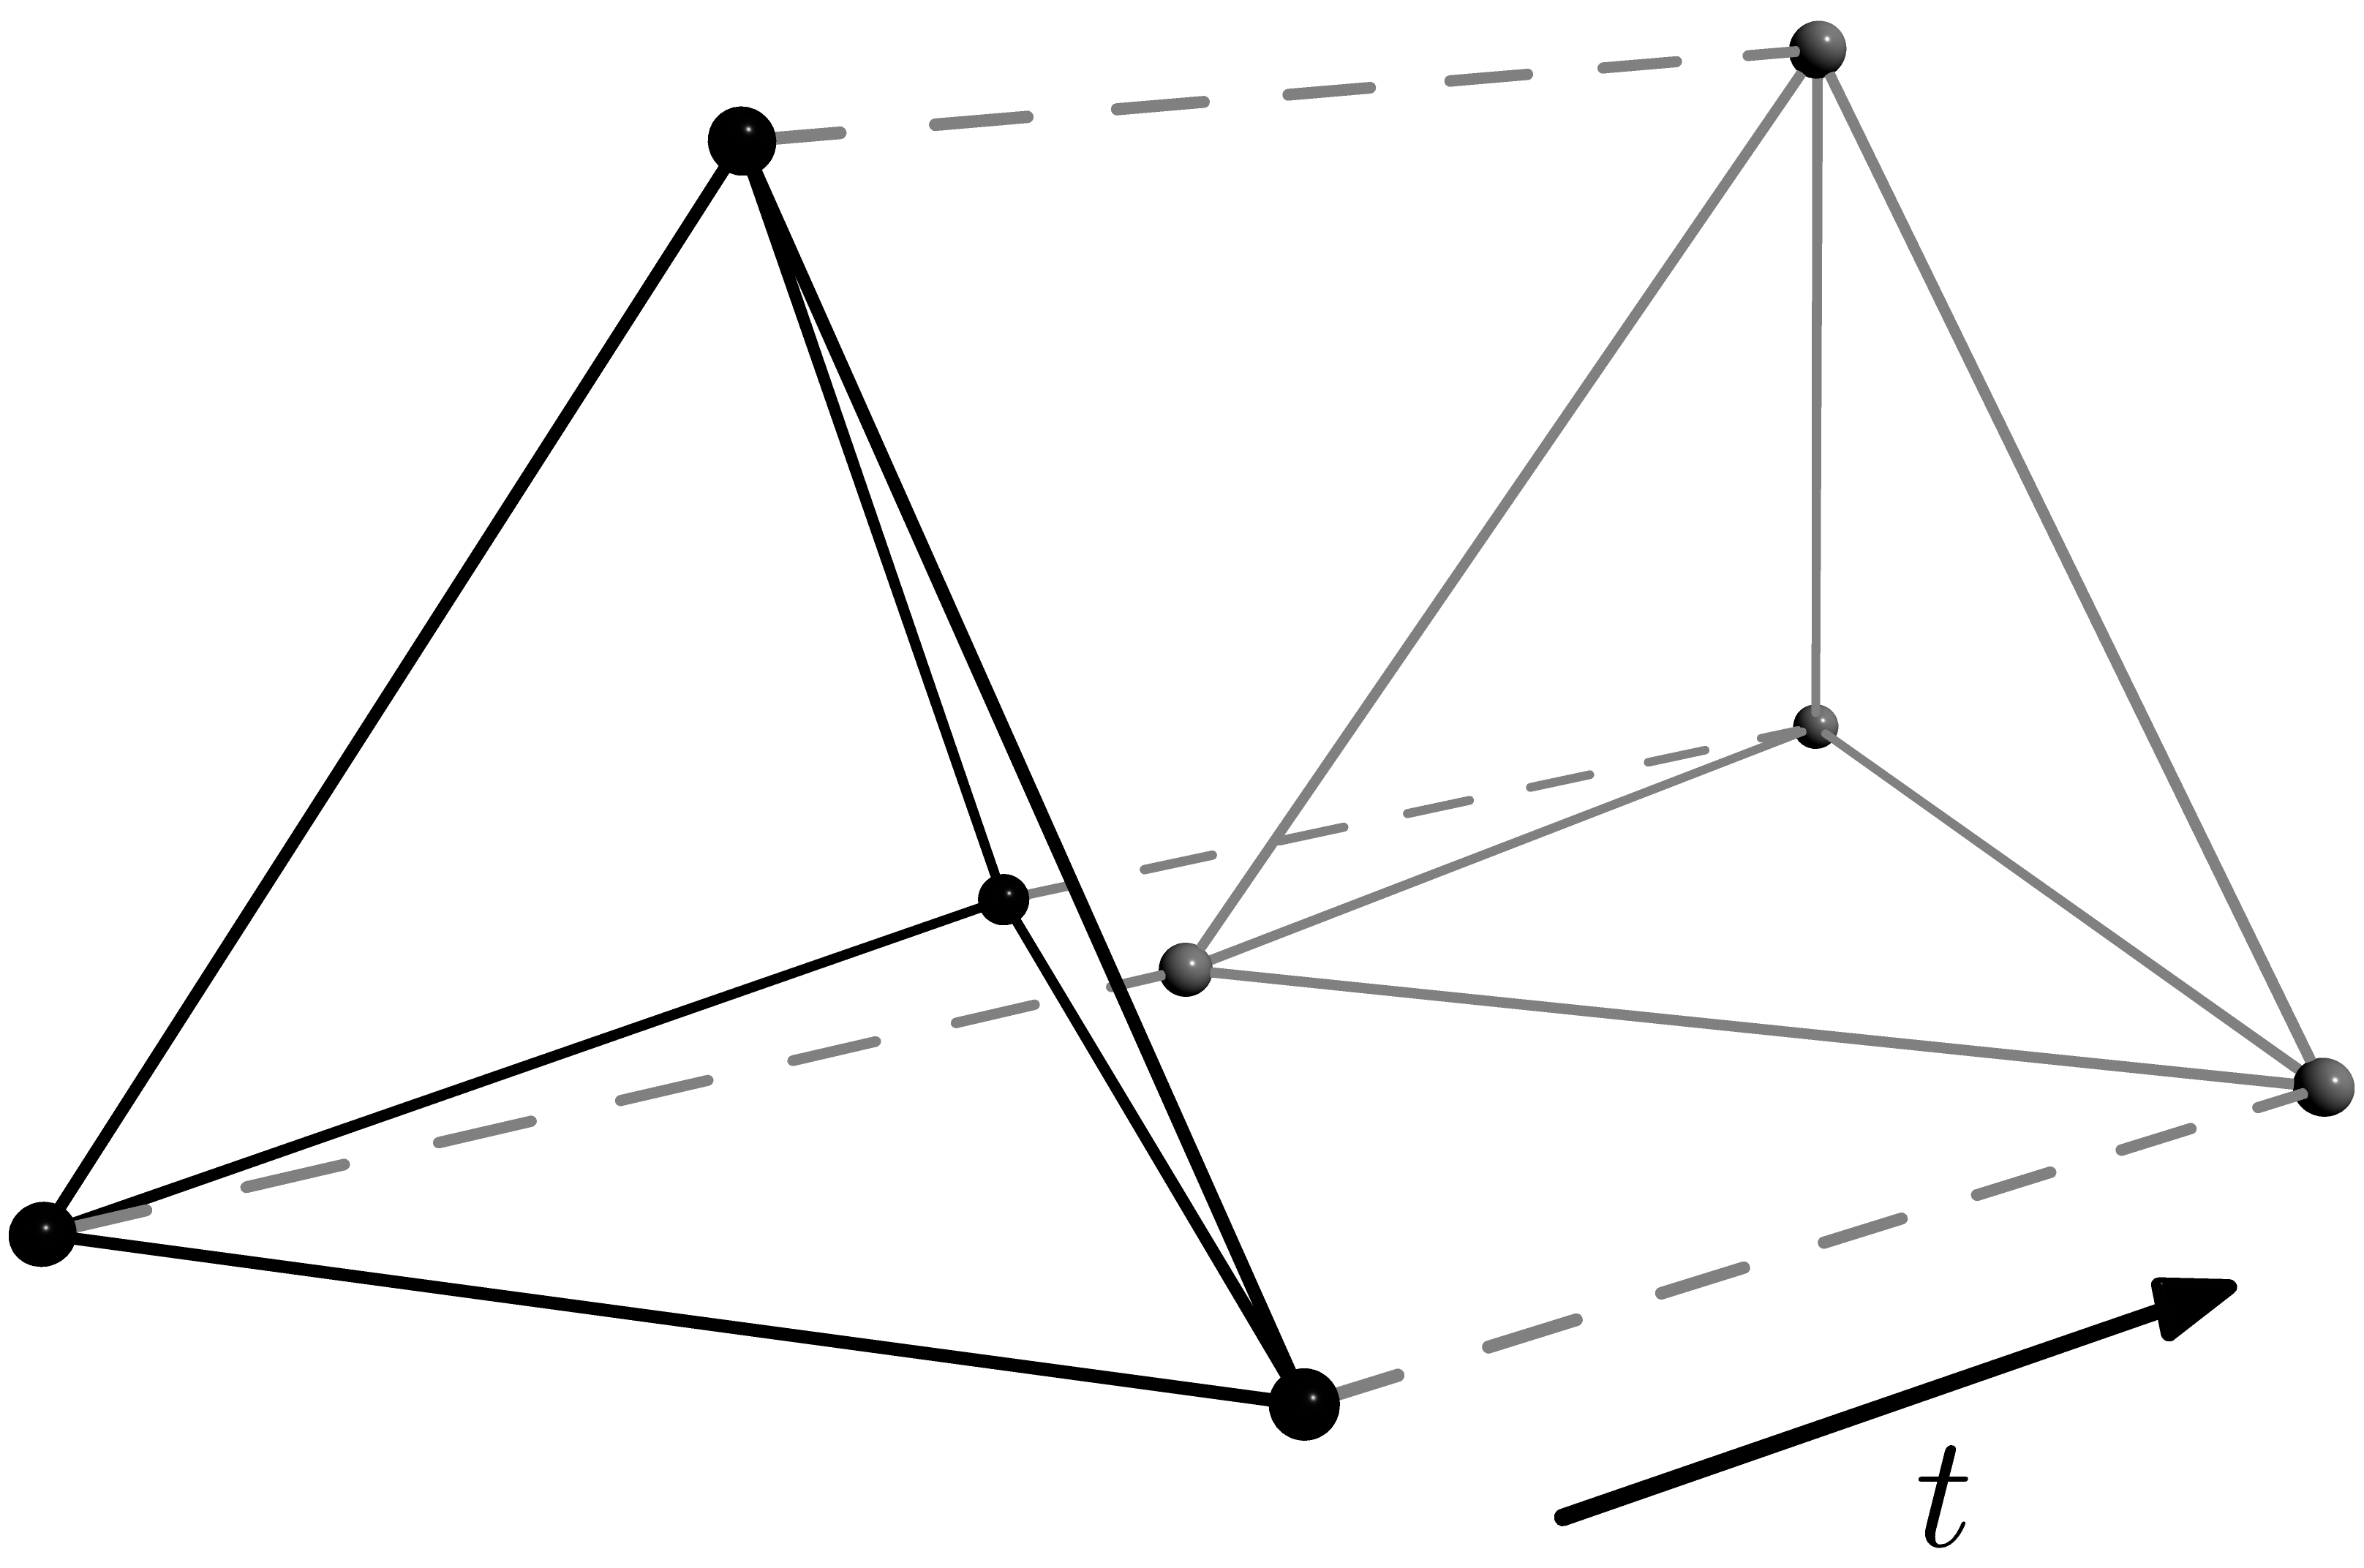
\includegraphics[width=0.4\textwidth]{figures/tetraprism_new.png}\label{fg:tet_domain}}
    \hspace{24pt}
    \subfloat[六面体柱积分域]{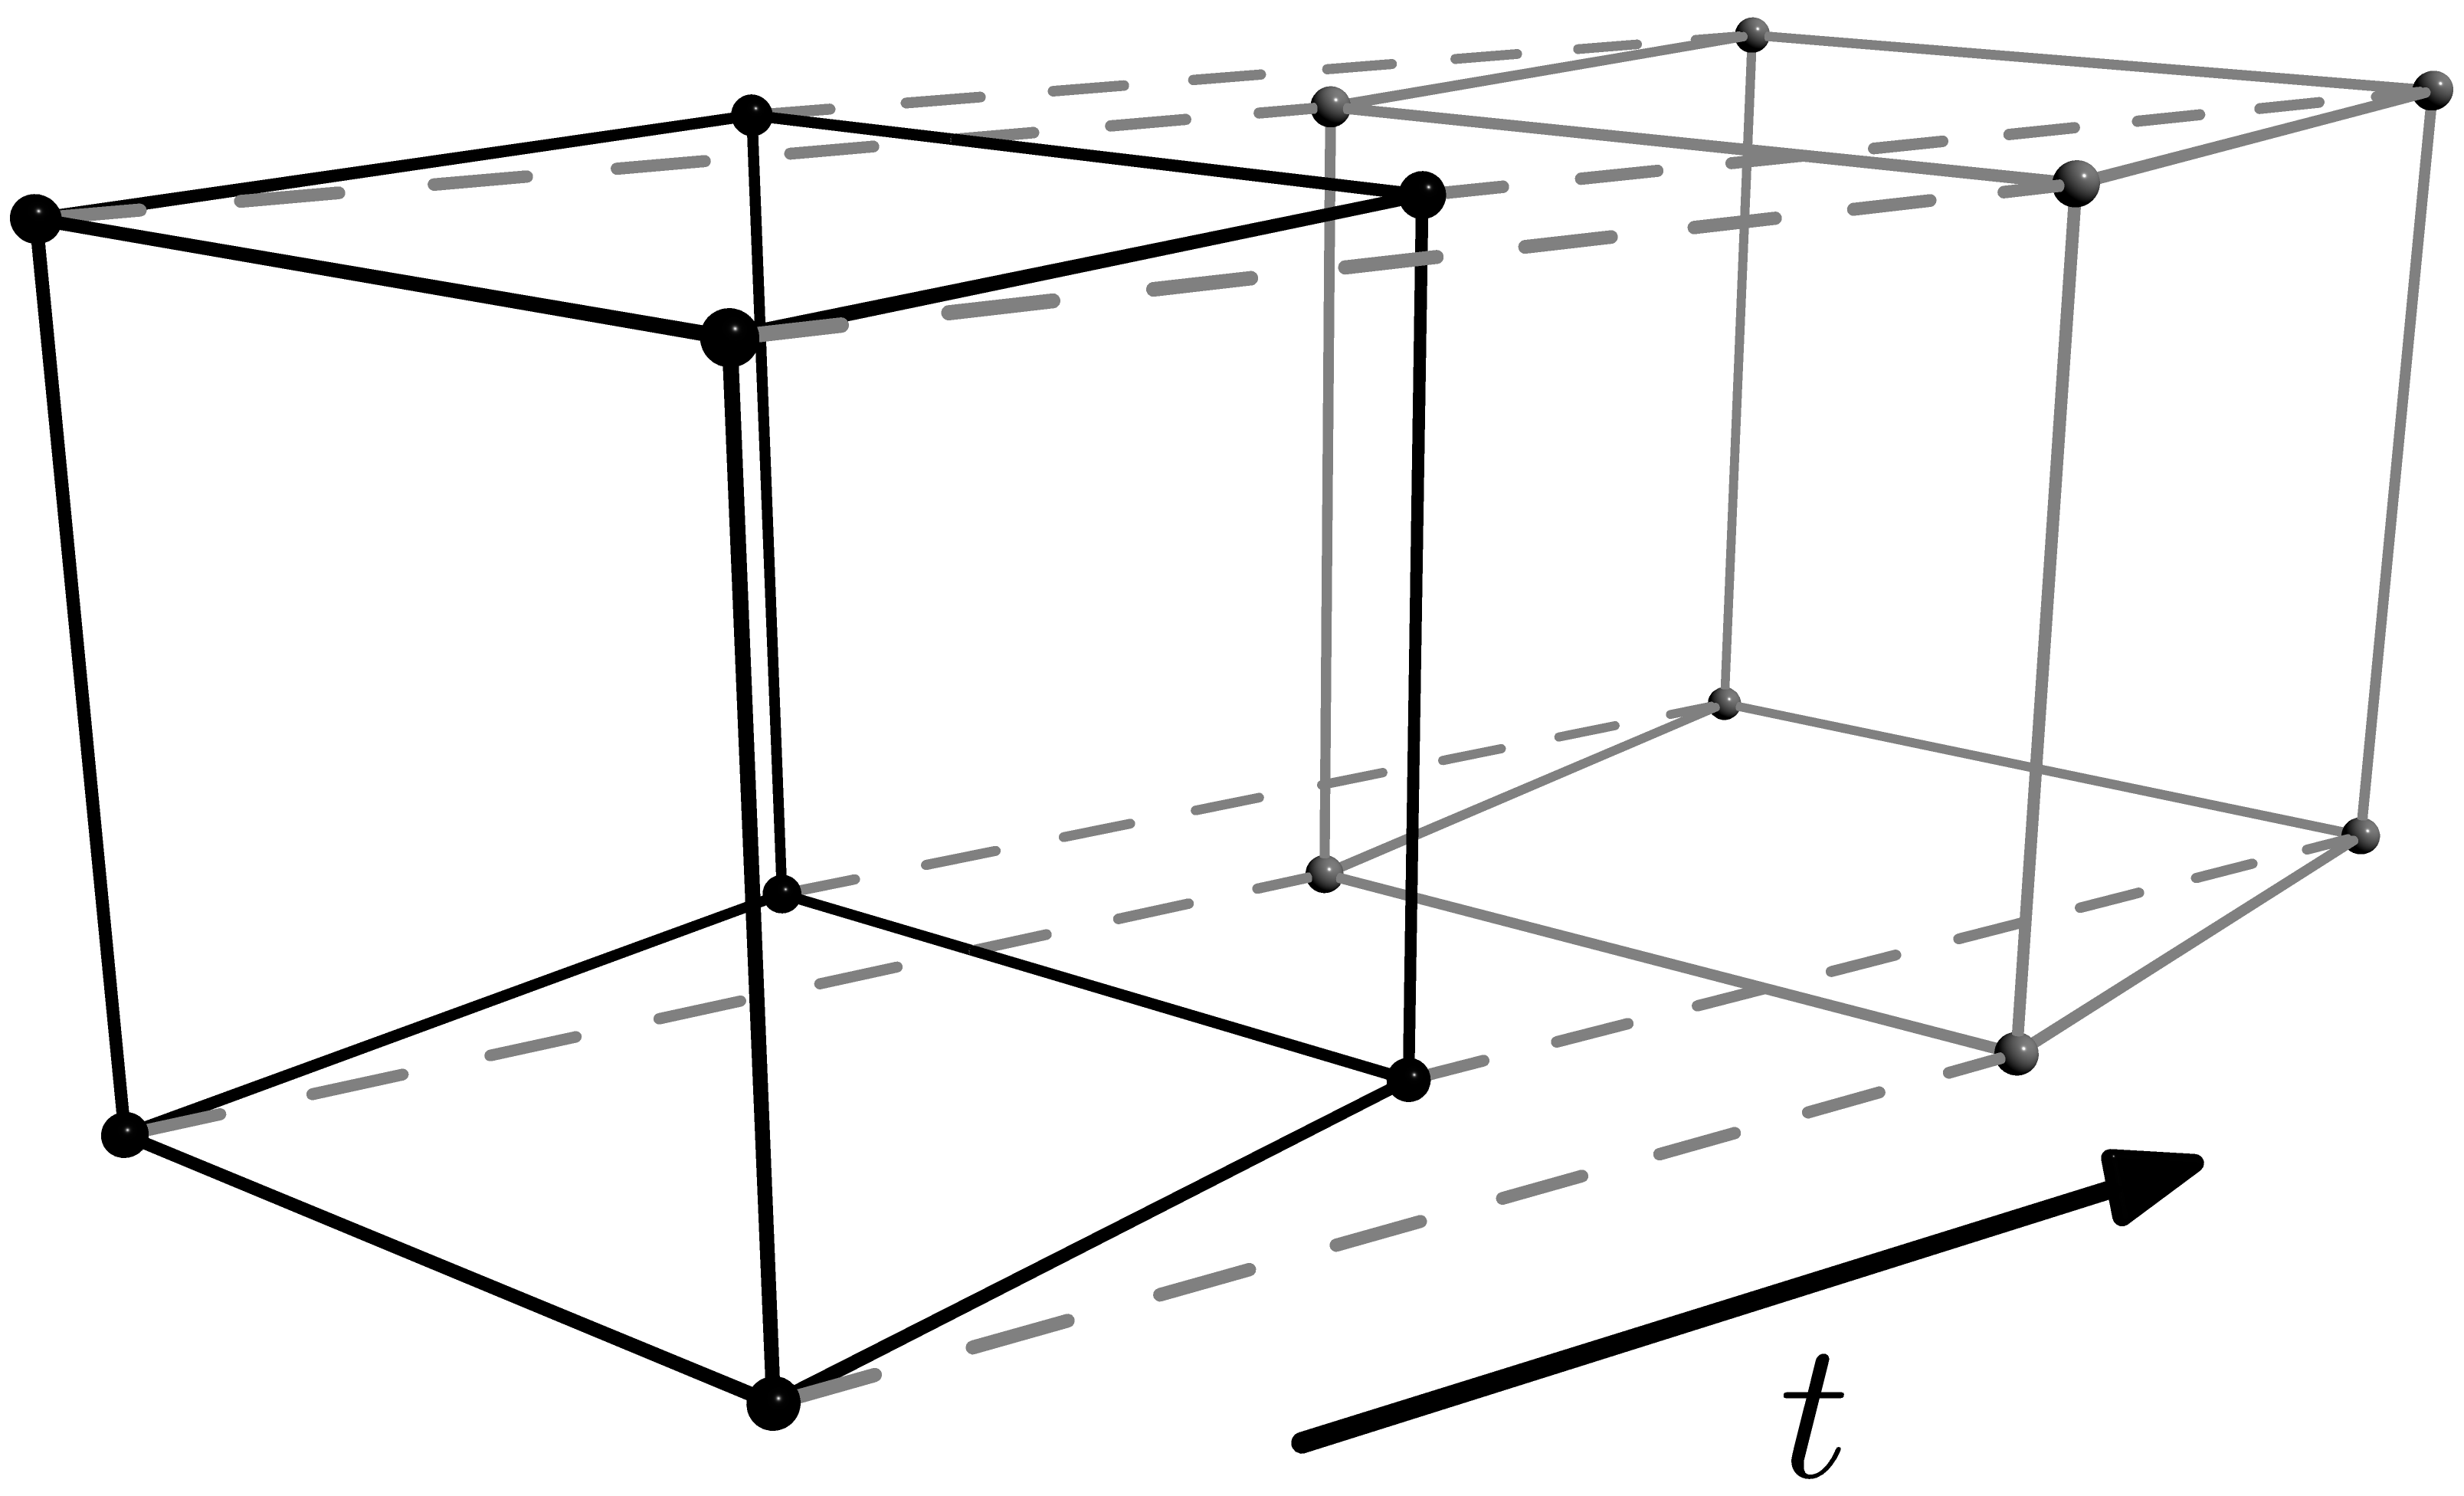
\includegraphics[width=0.4\textwidth]{figures/cubeprism_new.png}\label{fg:hex_domain}}
    \caption{四维空间背景积分域}
    \label{fg:domain}
\end{figure}

最后,通过分片试验验证所提数值积分方案是否满足变分一致性,同时利用典型波动问题测试其计算精度。

\subsubsection*{\bfseries (4)任意节点分布时空混合离散伽辽金无网格分析方法}
首先,将时空混合离散再生核无网格形函数及其光滑梯度引入拉格朗日乘子型伽辽金弱形式\eqref{eq:1}中,并采用优化的伽辽金无网格数值积分方案进行积分,得到相应的离散控制方程。
由式\eqref{eq:1} 可知,所提时空混合离散伽辽金弱形式中双线性算子均为同一算子,区别在于变量$u_h$和$p_h$所处的空间不一致。
造成空间不一致的原因在于$u_h$和$p_h$的本质边界条件不一致。当$u_h$和$p_h$采用相同的近似方式进行离散时,单独将施加本质边界条件部分的刚度矩阵分出,可得到如下所示离散控制方程:
\begin{equation}
    \begin{bmatrix} 
        \boldsymbol K + \boldsymbol K_{u} & \boldsymbol K \\
        \boldsymbol K & \boldsymbol K_{p} 
    \end{bmatrix} 
    \begin{Bmatrix}
        \boldsymbol u \\ \boldsymbol p
    \end{Bmatrix} =
    \begin{Bmatrix} \boldsymbol f_u \\ \boldsymbol f + \boldsymbol f_p \end{Bmatrix}
    \label{eq:3} 
\end{equation}
其中,$\boldsymbol K_u$和$\boldsymbol f_u$、$\boldsymbol K_p$和$\boldsymbol f_p$分别为施加与$u_h$和$p_h$相关的本质边界条件刚度矩阵和力向量。式\eqref{eq:3}中,刚度矩阵$\boldsymbol K$重复在三个地方使用,将利用该特点优化程序结构,降低内存开销。

同时,$u_h$与$p_h$的本质边界条件需要采用满足伽辽金法变分一致性的施加方案进行施加。本项目将在申请人所提基于Hellinger--Reissner原理伽辽金无网格本质边界条件施加方案的基础上,研究适用于拉格朗日乘子型时空混合离散伽辽金弱形式的变分一致型施加方案,确保全域的变分一致性。

随后,为进一步提升稳定性,将引入基于位移解梯度变化的自适应节点加密方案,对波的传播动态进行精确捕捉。同时,在求解离散控制方程时,拟嵌入基于Krylov子空间法的并行计算库,对程序进行提速。最后,通过典型波动问题和实际工程算例验证所提方法的有效性和可靠性。

\subsection{可行性分析}
针对制定的研究内容和研究目标,申请人对研究方案的每一部分进行项目的可行性分析,具体如下:

研究内容(1)拟基于拉格朗日乘子法建立适用于任意节点离散的时域末端虚位移本质边界条件。
该方案提供了一个全新的思路施加虚位移本质边界条件。
针对这部分研究内容的可行性,申请人采用一维杆结构动力问题对此研究方案进行初步验证。
不失一般性,问题的空间区域与时间区域所构成的二维时空区域采用均布的线性三角形有限元单元进行离散,图 \subref*{fg:bar_2} 为位移云图,从图中可以看出在均布节点的离散情况下,拉格朗日乘子型时空混合伽辽金弱形式无需分块网格技术,即可得到稳定的数值结果。
图 \subref*{fg:bar_3} 为该问题的位移云图和位移误差收敛率分析,从图中可以看出该混合离散框架可以保证理论误差收敛率。
但是,当时间区域节点间距过大时,数值色散问题将导致计算结果出现振荡现象,需要本项目后续研究内容的成果解决此问题。从拉压杆动力测试当中可以初步数值验证所提研究方案可行,后续可在此基础上,延续制定的研究方案逐步完善该方法的理论基础,达成所提研究目标。

\begin{figure}[!h]
    \centering 
    % \includegraphics[width=2cm]{figures/cubeprism.png}
    % \subcaptionbox{\includegraphics{figures/cubeprism.png}}
    \subfloat[问题模型与精确解]{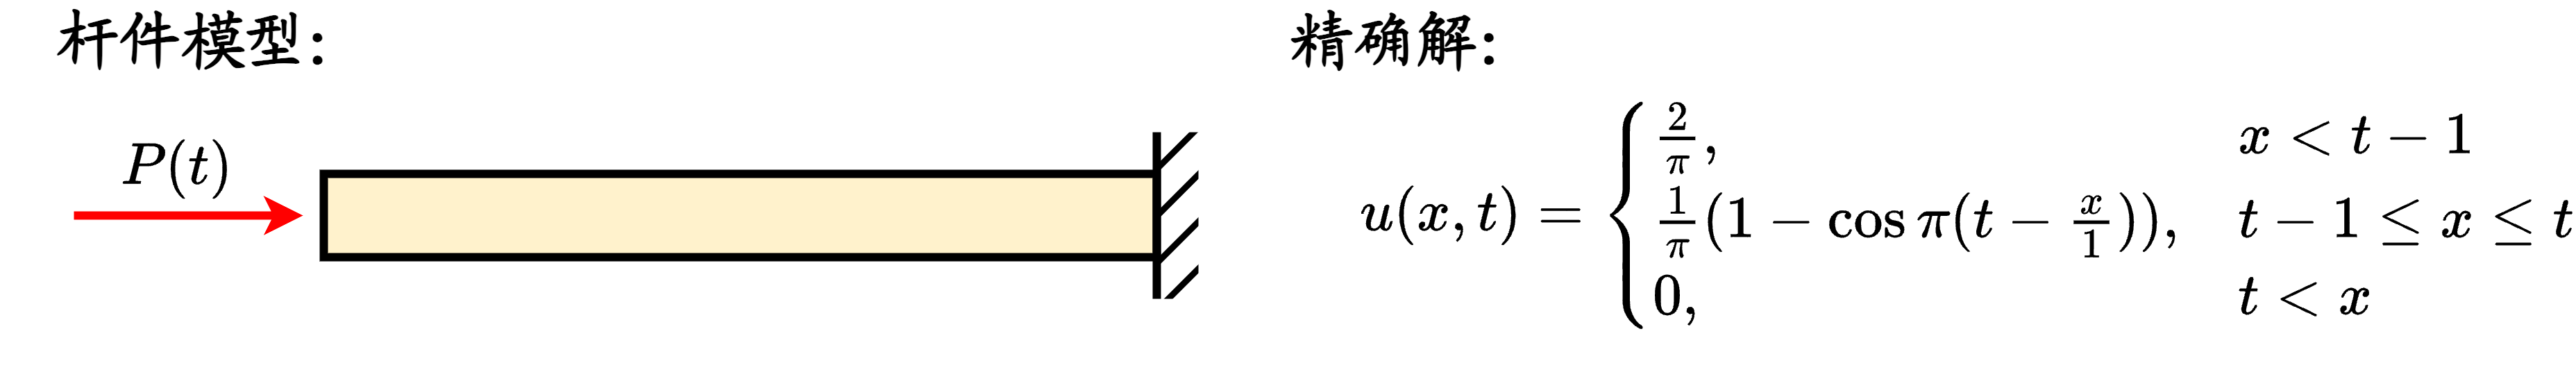
\includegraphics[width=\textwidth]{figures/bar.png}\label{fg:bar_1}}

    \subfloat[位移云图]{
\includegraphics[width=0.50\textwidth]{figures/bar_contour.png}\label{fg:bar_2}}
    % \hspace{24pt}
    \subfloat[误差收敛率分析]{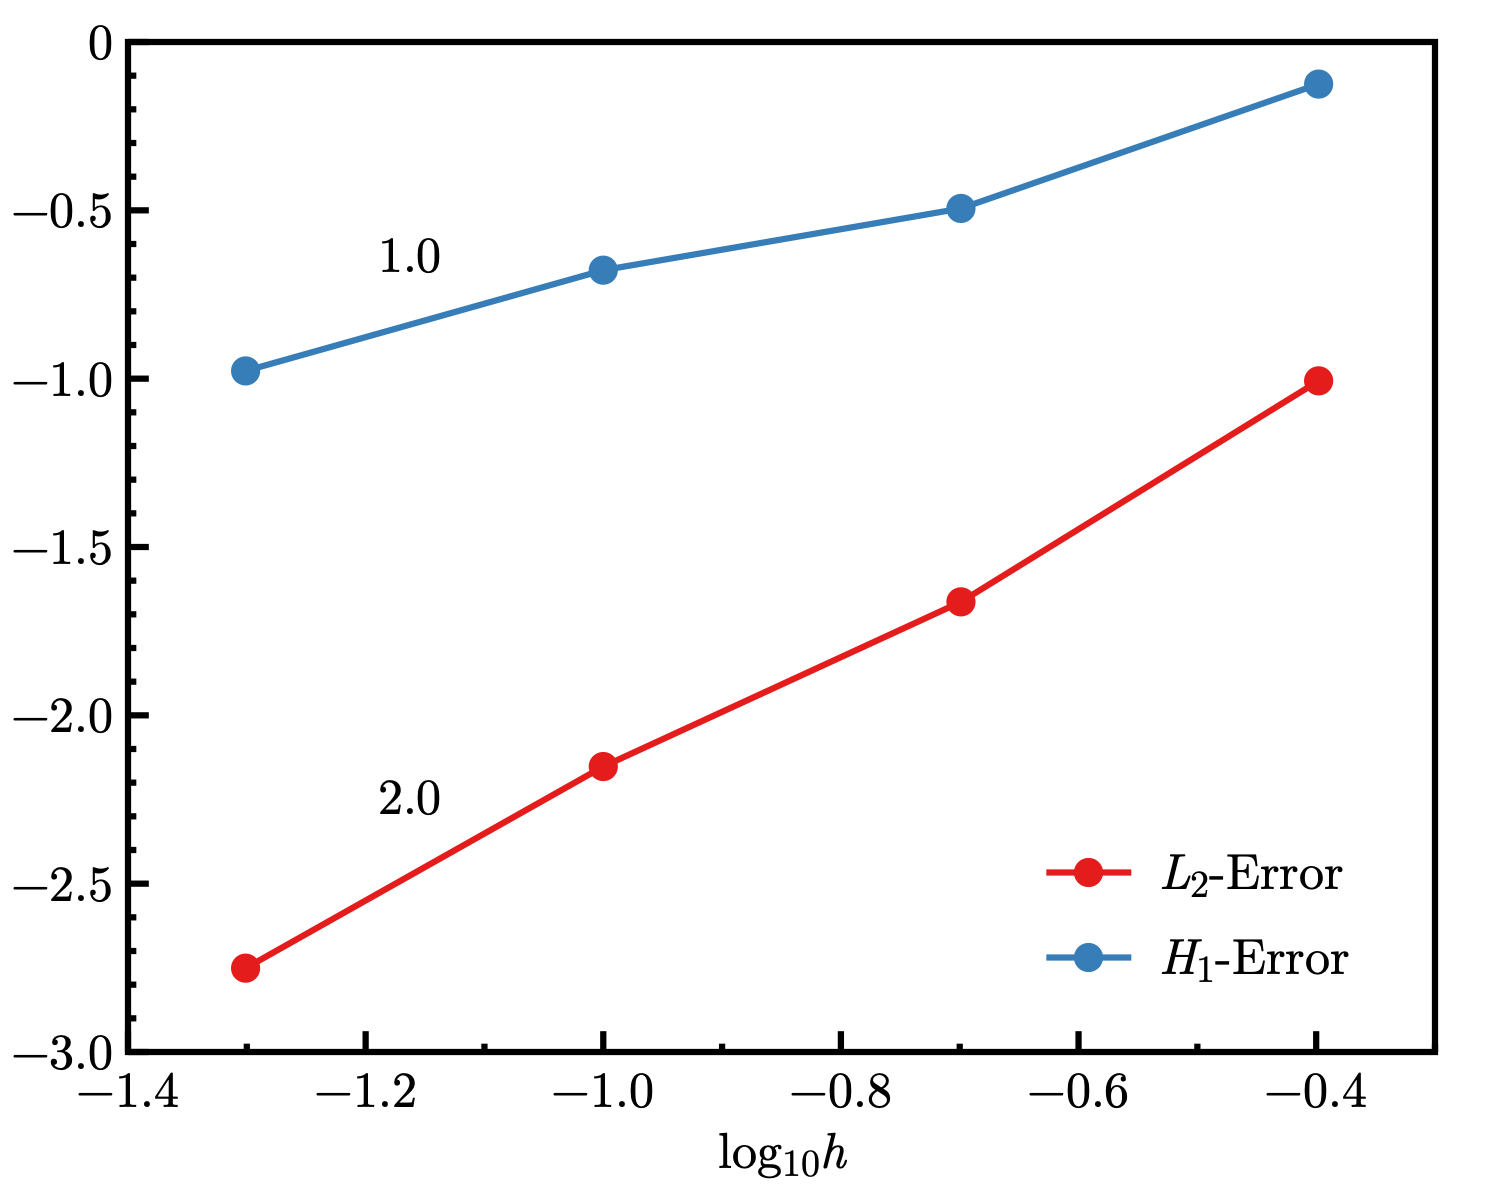
\includegraphics[width=0.50\textwidth]{figures/error.png}\label{fg:bar_3}}
    \caption{拉格朗日型虚位移边界条件施加方案初步测试:杆结构动力问题}
    \label{fg:bar}
\end{figure}

研究内容(2)拟建立可缓解数值色散现象的再生核无网格近似方案。
该方案通过对时空混合离散伽辽金法进行局部截断误差估计,确定时间域和空间域混合离散的近似阶次。
并利用再生核无网格近似,构造相对应阶次的时空混合离散形函数。
针对伽辽金无网格法误差分析方面,申请人已对伽辽金无网格法的正交性条件\cite{wu2021}和动力分析中的频率\cite{wu2018a}提出了相应的误差估计。
尤其是动力分析中的频率误差估计,建立该估计所采用的方法与本项目研究方案(2)中拟采用的方案一致,均为基于特征解的局部截断误差估计的方法,在一定程度上说明此研究方案可行。
在时空混合离散再生核近似方面,申请人在构造非常规基向量再生核近似形函数也具有一定的研究经验,
曾针对Helmholtz方程提出基于三角函数基向量的再生核近似\cite{wang2020b}。
而Helmholtz方程也是本项目研究波动问题稳态解的控制方程。
相关研究成果支持研究方案(2)可行。

研究内容(3)拟在时空混合离散伽辽金弱形式中引入再生光滑梯度无网格数值积分方案进行求解,并利用数值积分点在积分域间的共享特性优化全局积分点数,提升计算效率。
申请人针对高阶伽辽金无网格数值积分过程提出了嵌套子域积分法\cite{wang2016b}和再生光滑梯度积分法\cite{wang2019a},再生光滑梯度积分法也是本研究内容拟采用的方法。
该方法是基于假定应变理论变分一致型无网格数值积分方案的通用理论框架,适用于任意形式基向量的无网格形函数,如研究方案(2)所提时间域与空间域不同阶次的基函数。
在再生光滑梯度理论框架下,伽辽金无网格法采用与基函数阶次相对应的数值积分方案即可满足积分约束条件,保证计算精度。同时,该框架支持针对伽辽金弱形式中的背景积分域积分和边界积分优化积分点数量,提升计算效率。申请人与合作者还将该方法推广至相场断裂模型分析\cite{wu2020a}、Helmholtz问题分析\cite{wang2020b}、薄板壳问题\cite{wu2023,wu2024}、动力分析\cite{Fu2022}和应变梯度问题\cite{du2022},系列工作说明本研究内容具可行性。

研究内容(4)拟建立时空混合离散伽辽金无网格法,该方法需要结合研究内容(1--3)中所提的时域末端虚位移本质边界条件施加方案、时空混合离散再生核无网格近似方案、时空混合离散变分一致型伽辽金无网格数值积分方案,并引入基于位移解梯度变化的自适应节点加密方案和求解线性方程组的并行计算库,提升方法的精度和效率。
在该方法建立过程中,本质边界条件施加方案需进一步改进,使其满足变分一致性。
申请人基于Hellinger--Reissner和Hu--Washizu多变量变分原理提出了弹性力学、薄板和薄壳问题的变分一致型伽辽金无网格法本质边界条件施加方案\cite{Wu2022b,wu2023,wu2024}。
该方法不仅完备了再生光滑梯度积分法的理论基础,并且能保证整体伽辽金法的变分一致性,且无需额外稳定项和人工经验参数。
该方法也是本研究方案计划采用方法,相关研究成果支持本研究方案的可行性。
其次,基于位移解梯度变化的自适应节点加密方案和线性方程组并行求解方案都是较为成熟的技术方法,没有特别的技术障碍,不影响本研究内容的可行性。

综上所述,申请人就本项目的关键科学问题和研究方案中的关键步骤的相关内容进行了系列研究,取得了一定的研究成果,为本项目的研究提供了坚实的基础。鉴于以上分析,本项目所提的研究方案具有很强的可行性。


\end{MS}

\section{\textbf{本项目的特色与创新之处;}}

\begin{MS}
	
本项目的特色与创新之处包括以下三点:

\begin{enumerate}[label=(\theenumi),left=24pt]
    \item 时域末端虚位移本质边界条件施加方案
    实现了基于弱形式施加虚位移本质边界条件,无需分块网格划分,即可保证求解的稳定性。同时始末节点也无需匹配个数,降低节点离散的要求。
    \item 时空混合离散无网格近似方案利用再生核近似构造高阶形函数的便利性,在任意节点离散情况下即可缓解数值色散问题。基于节点离散的再生核近似局部节点加密过程实现简单,无需考虑几何拓扑关系。
    \item 在时域末端虚位移本质边界条件施加方案、时空混合离散无网格近似方案的协同作用下,时空混合伽辽金无网格分析方法可适用于任意节点离散情况,并且能轻松地进行局部区域的节点加密,更好捕捉波动问题的局部特征。
\end{enumerate}

\vspace{24pt}

\end{MS}

\section{\textbf{年度研究计划及预期研究结果}\kg{0.2em}(包括拟组织的重要学术交流活动、国际合作与交流计划等)。}

\begin{MS}
	\subsection{年度研究计划}
本项目围绕拟定的研究目标,通过理论推导和数值验证的方法研究任意节点分布的时空混合离散伽辽金无网格法。
根据各部分研究内容的逻辑关系,制定了表 \ref{tb:plan} 所示的项目的年度计划表。
其中,成果整理、论文发表及年度报告贯穿执行期。
项目参与人执行期内计划参加学术会议并作项目相关报告不少于每年2人次。

\begin{table}[!h]
\caption{年度研究计划表}\label{tb:plan}
\centering
\begin{ganttchart}[
    % inline,
    % bar inline label anchor = north,
    include title in canvas=false,
    x unit = 8pt,
    y unit title = 14pt,
    hgrid={*1{draw=black!5, line width=.75pt}},
    vgrid={*1{draw=black!5, line width=.75pt}},
    canvas/.append style={fill=none,draw=black!20,line width=.75pt},
    title/.style={draw=black!5, fill=none},
    title height=1,
    bar height = 0.3,
    group height=.1,
    % title label node/.append style={below=0pt},
    newline shortcut=true,
    % bar label node/.append style={align=left, anchor=north},
    bar/.append style={fill=blue!50, rounded corners=4pt, draw=none},
    group label node/.append style={align=left, left=-.5cm, text width=17em},
    bar label node/.append style={left=0cm,align=left,text width=15em},
]{1}{32}
    \gantttitle{2026}{8}
    \gantttitle{2027}{8}
    \gantttitle{2028}{8}
    \gantttitle{2029}{8} \\
    \gantttitle{上半年}{4}
    \gantttitle{下半年}{4}
    \gantttitle{上半年}{4}
    \gantttitle{下半年}{4}
    \gantttitle{上半年}{4}
    \gantttitle{下半年}{4}
    \gantttitle{上半年}{4}
    \gantttitle{下半年}{4} \\
    \ganttgroup{\bfseries 研究内容(1)}{1}{8} \\
    \ganttbar{查阅相关文献,测试不同虚位移边界条件时空混合离散伽辽金法性能}{1}{4}\\
    \ganttbar[name=scheme1]{研究拉格朗日乘子型时域末端虚位移本质边界条件施加方案}{3}{8}\\
    \ganttgroup{\bfseries 研究内容(2)}{9}{20} \\
    \ganttbar[name=error]{推导稳定性分析局部截断误差估计}{9}{20} \\
    \ganttbar[name=scheme2]{构建时空混合离散再生核近似方案}{13}{16} \\
    \ganttgroup{\bfseries 研究内容(3)}{17}{26} \\
    \ganttbar[name=scheme3]{推导时空混合离散再生光滑梯度}{17}{24} \\
    \ganttbar[name=scheme4]{优化四维积分域再生光滑梯度积分方案}{21}{26} \\
    \ganttgroup{\bfseries 研究内容(4)}{21}{28} \\
    \ganttbar[name=method]{构建时空混合离散伽辽金无网格法}{21}{24} \\
    \ganttbar{引入自适应节点分布算法和并行计算优化程序}{23}{28} \\
    \ganttbar{成果整理、论文发表、软件著作权申请、年度报告及项目结题报告}{5}{32}
\end{ganttchart}
\end{table}

\subsection{预期研究结果}
本项目预期取得如下研究结果:

\begin{enumerate}[label=(\theenumi),left=24pt]
    \item 时空混合离散伽辽金法时域末端本质边界条件施加方案;
    \item 免数值色散问题的时空混合离散再生核无网格近似方案;
    \item 任意节点分布的混合离散高效伽辽金无网格分析方法;
    \item 在计算力学领域重要期刊发表论文5--9篇,申请软件著作权1项;
    \item 培养研究生不少于4名。
\end{enumerate}

\newpage
\end{MS}

\chapter{\textbf{研究基础与工作条件}}
\section{\textbf{研究基础}\kg{0.2em}(与本项目相关的研究工作积累和已取得的研究工作成绩);}

\begin{MS}
	

项目申请人主要从事伽辽金无网格法相关领域研究,并取得了一定的研究成果,已有国内外计算力学领域重要期刊发表论文20余篇,其中5篇发表于\textit{Computer Methods in Applied Mechanics and Engineering}。
相关系列工作不仅为本项目的研究奠定了坚实的研究基础,并积累了丰富的理论分析经验。具体的系列工作如下:

\subsubsection*{\bfseries (1)变分一致型伽辽金无网格法本质边界条件施加方案}
通常情况下,无网格近似形函数通常不具备插值性,无法直接施加本质边界条件,需通过基于弱形式的方案进行施加。
同时,变分一致型伽辽金无网格法也需要变分一致的本质边界条件施加方案配合,️以满足全域变分一致性。
针对该问题,申请人基于Hellinger--Reissner(HR)多变量变分原理发展了新型伽辽金无网格法本质边界条件施加方案。
该方法具有与传统Nitsche本质边界条件施加方法具有相类似的格式,同样具有一致项和稳定项。
图 \ref{fg:plate} 为所提方法在简支三角形方板问题中与传统罚函数法(Penalty)、Nitsche法的计算效率对比和人工参数敏感性分析。
相较于Nitsche法,所提方法一致项采用形函数的光滑导数替代传统无网格形函数高阶导数,在保证变分一致性的同时提高计算效率。
因此,在图 \subref*{fg:plate_time} 中所提HR方法在计算形函数及其导数上计算耗时大幅少于Nitsche,并于罚函数法相当。
而稳定项自然存在于所提方法弱形式中,无需额外引入稳定项,且稳定项中也不存在人工经验参数。
图 \subref*{fg:plate_alpha} 为计算精度和人工参数的关系,从图中可以看出,罚函数法和Nitsche法随人工参数取值不同,计算精度也随之改变。
取得最优精度时的人工参数在不同节点离散下也不相同,而所提HR型本质边界条件施加方案无需人工经验参数,即可达到传统方法的最优计算精度,使用过程简单方便。
此外,申请人还基于Hu--Washizu变分原理将该方法推广至薄壳问题中,发展薄壳结构准变分一致伽辽金无网格分析方法。

上述变分一致型伽辽金无网格法本质边界条件施加方案,为本项目研究时空混合离散伽辽金法时域末端虚位移本质边界条件施加方案奠定的重要的研究基础。

\begin{figure}[!h]
    \centering 
    \subfloat[计算效率对比]{\includegraphics[width=0.444\textwidth]{figures/HRplate_time.png}\label{fg:plate_time}}
    \subfloat[人工参数$\alpha$敏感性分析]{\includegraphics[width=0.546\textwidth]{figures/HRplate_alpha.png}\label{fg:plate_alpha}}
    \caption{HR变分一致型伽辽金无网格本质边界条件施加方案对比传统方案}
    \label{fg:plate}
\end{figure}

系列工作研究成果如下:

\vspace{-50pt}
\begin{thebibliography}{1}
	\bibitem[Wu et~al.(2024)Wu, Xu, Xu, and Basha]{hw2024}
	\textul{\textbf{Wu J}}, Xu Y, Xu B, Basha S~H.
	\newblock Quasi-consistent efficient meshfree thin shell formulation with
	  naturally stabilized enforced essential boundary conditions.
	\newblock \emph{Engineering Analysis with Boundary Elements}, 2024, 163:
	  641-655.

	\bibitem[Wu et~al.(2023)Wu, Wu, Zhao, and Wang]{hr2023}
	\textul{\textbf{Wu J}}, Wu X, Zhao Y, Wang D.
	\newblock A rotation-free {{Hellinger-Reissner}} meshfree thin plate
	  formulation naturally accommodating essential boundary conditions.
	\newblock \emph{Engineering Analysis with Boundary Elements}, 2023, 154:
	  122-140.

	\bibitem[吴俊超\ 等(2022)吴俊超, 吴新瑜, 赵珧冰, and
	  王东东]{hr2022}
	\textul{\textbf{吴俊超}}, 吴新瑜, 赵珧冰, 王东东.
	\newblock
	  {基于赫林格-赖斯纳变分原理的一致高效无网格本质边界条件施加方法}.
	\newblock 力学学报, 2022, 54: 3283-3296.

\end{thebibliography}

\subsubsection*{\bfseries (2)伽辽金无网格法精度分析}
由于无网格形函数的有理特性,伽辽金无网格法误差估计中将不可忽略由数值积分不准确引起的精度损失。
申请人采用泛函分析的手段,首次将变分一致性条件与伽辽金法正交性条件建立联系。
分析由数值积分满足变分一致性条件阶次和计算误差之间的关系,建立考虑数值积分误差的伽辽金无网格法误差估计。
该误差估计表达式分为两部分,一部分由形函数一致性条件确定,另一部分则由变分一致性条件控制。
该误差估计揭示了用于测试变分一致性条件的经典分片试验是如何影响计算误差。
图 \ref{fg:cube} 为三维方块势问题的伽辽金无网格法误差估计表达式的数值验证,算例中采用了满足变分一致性的再生核光滑梯度积分无网格法(RKGSI)和不满足变分一致性的高斯积分无网格法(GI)进行对比。
从分片试验图 \subref*{fg:cube_contour} 可以看出,仅有满足变分一致性的再生光滑梯度积分无网格法可通过分片试验,即使采用20点高斯积分(GI-20),传统方法依旧存在不可忽略误差。图 \subref*{fg:cube_slope} 为误差收敛率分析,该图可用所提伽辽金无网格法误差估计解释。当节点间距较大时,误差收敛率由一致性条件控制,高斯积分法可达到理论误差收敛率。当节点间距进一步加密,由一致性条件控制的误差迅速减小,高斯积分法误差收敛率转为由变分一致性条件控制而降低。再生光滑梯度理论框架可使两部分误差阶次保持一致,始终保持最优误差收敛效果。

\begin{figure}[!h]
    \centering 
    \subfloat[分片试验]{\includegraphics[width=0.45\textwidth]{figures/cube_contour.png}\label{fg:cube_contour}}
    \subfloat[误差收敛率分析]{\includegraphics[width=0.55\textwidth]{figures/cube_slope.png}\label{fg:cube_slope}}
    \caption{伽辽金无网格法误差估计验证}
    \label{fg:cube}
\end{figure}

另一方面,申请人针对波动问题伽辽金无网格法振动分析,建立频率的局部截断误差估计表达式。
该误差估计表达式详细分析了如图 \subref*{fg:frequency_shape} 所示无网格形函数的周期性条件,并引入基于特征解的节点系数和形函数一致性条件进行化简。
基于此误差估计,将一致质量矩阵与局部质量矩阵进行优化组合,以消除低阶误差项,得到伽辽金无网格频率分析的高阶质量矩阵。
图 \subref*{fg:frequency_mass} 为高阶质量矩阵无网格法(HOM)与传统一致质量矩阵无网格法(CM)的频谱分析,结果表明高阶质量矩阵无网格法在波传播的任意方向上计算误差均优于一致质量矩阵伽辽金无网格法。

申请人在伽辽金无网格法误差估计中的研究结果,为本项目解决关键科学问题(2)如何确定时空混合无网格近似基向量阶次对求解稳定性的影响机理,提供了理论基础框架。
值得注意的是,频率局部截断误差估计中所采用的方案也是推导时空混合离散伽辽金无网格法局部截断误差估计中拟采用的研究方案。

\begin{figure}[!h]
    \centering 
    \subfloat[无网格形函数周期性]{\includegraphics[width=0.7\textwidth]{figures/shape.png}\label{fg:frequency_shape}}
    \subfloat[无网格法频谱分析]{\includegraphics[width=0.3\textwidth]{figures/mass.png}\label{fg:frequency_mass}}
    \caption{伽辽金无网格法频率误差估计验证}
    \label{fg:frequency}
\end{figure}


系列工作研究成果如下:

\vspace{-50pt}
\begin{thebibliography}{1}
	\bibitem[Wu et~al.(2021)Wu and Wang]{accuracy2021}
	\textul{\textbf{Wu J}}, Wang D.
	\newblock An accuracy analysis of {{Galerkin}} meshfree methods accounting for
	  numerical integration.
	\newblock \emph{Computer Methods in Applied Mechanics and Engineering}, 2021,
	  375: 113631.

	\bibitem[Wu et~al.(2018)Wu, Wang, and Lin]{mass2018}
	\textul{\textbf{Wu J}}, Wang D, Lin Z.
	\newblock A meshfree higher order mass matrix formulation for structural
	  vibration analysis.
	\newblock \emph{International Journal of Structural Stability and Dynamics},
	  2018, 18: 1850121.

\end{thebibliography}

\subsubsection*{\bfseries (3)变分一致型伽辽金无网格数值积分方案}
为解决伽辽金无网格法无法满足变分一致性引起精度下降问题,申请人发展了嵌套子域法和再生光滑梯度积分法。
尤其是再生光滑梯度积分法,该方法理论框架涵盖了所有以假定应变为基础的变分一致型数值积分方案。
在此框架下,采用与无网格基函数阶次配套的数值积分方案即可满足变分一致性。
同时,该框架还支持利用数值积分点在域积分和边界积分中的共享特性,对全域积分点数量进行优化,提高计算效率。
该方法经过近几年的发展,成功应用到了动力问题分析、Helmholtz方程分析、应变梯度结构分析、相场断裂模型分析等问题中。
本项目研究方案中拟将再生光滑梯度积分法推广应用至时空混合离散伽辽金无网格分析当中,以满足时空混合离散伽辽金弱形式的变分一致性,保证计算精度。
同时,将利用再生光滑梯度理论框架的优势,进一步优化四维时空区域数值积分点数量,提高整体分析的计算效率。

上述变分一致型伽辽金无网格数值积分方案的系列工作,为本项目研究时空混合离散伽辽金无网格法提供了扎实的理论基础。

系列工作研究成果如下:

\vspace{-50pt}
\begin{thebibliography}{1}
	\bibitem[Wang et~al.(2019)Wang and Wu]{RKGSI2019}
	Wang D, \textul{\textbf{Wu J}}.
	\newblock An inherently consistent reproducing kernel gradient smoothing
	  framework toward efficient {{Galerkin}} meshfree formulation with explicit
	  quadrature.
	\newblock \emph{Computer Methods in Applied Mechanics and Engineering}, 2019,
	  349: 628-672.

	\bibitem[Wang et~al.(2016)Wang and Wu]{NSGSI2016}
	Wang D, \textul{\textbf{Wu J}}.
	\newblock An efficient nesting sub-domain gradient smoothing integration
	  algorithm with quadratic exactness for {{Galerkin}} meshfree methods.
	\newblock \emph{Computer Methods in Applied Mechanics and Engineering}, 2016,
	  298: 485-519.

	\bibitem[Wu et~al.(2020)Wu, Wang, Lin, and Qi]{PF2020}
	\textul{\textbf{Wu J}}, Wang D, Lin Z, Qi D.
	\newblock An efficient gradient smoothing meshfree formulation for the
	  fourth-order phase field modeling of brittle fracture.
	\newblock \emph{Computational Particle Mechanics}, 2020, 7: 193-207.

	\bibitem[Wang et~al.(2020)Wang, Wu, and Wang]{Helmholtz2020}
	Wang J, \textul{\textbf{Wu J}}, Wang D.
	\newblock A quasi-consistent integration method for efficient meshfree analysis
	  of {{Helmholtz}} problems with plane wave basis functions.
	\newblock \emph{Engineering Analysis with Boundary Elements}, 2020, 110: 42-55.

	\bibitem[吴俊超\ 等(2016)吴俊超, 邓俊俊, 王家睿, and
	  王东东]{integration2016}
	\textul{\textbf{吴俊超}}, 邓俊俊, 王家睿, 王东东.
	\newblock 伽辽金型无网格法的数值积分方法.
	\newblock 固体力学学报, 2016, 3: 208-233.

	\bibitem[Du et~al.(2022)Du, Wu, Wang, and Chen]{RKGSIgradient2022}
	Du H, \textul{\textbf{Wu J}}, Wang D, Chen J.
	\newblock A unified reproducing kernel gradient smoothing {{Galerkin}} meshfree
	  approach to strain gradient elasticity.
	\newblock \emph{Computational Mechanics}, 2022, 70: 73-100.

	\bibitem[付赛赛\ 等(2022)付赛赛, 邓立克, 吴俊超, 王东东, and
	  张灿辉]{RKGSIdynamic2022}
	付赛赛, 邓立克, \textul{\textbf{吴俊超}}, 王东东, 张灿辉.
	\newblock 再生光滑梯度无网格法动力特性研究.
	\newblock 应用力学学报, 2022, 39: 1065-1075.

\end{thebibliography}

综上所述,项目申请人及其团队在伽辽金无网格法的系列工作为本项目的顺利开展提供了良好的研究基础。


\end{MS}

\section{\textbf{工作条件}\kg{0.2em}(包括已具备的实验条件,\kg{0.2em}尚缺少的实验条件和拟解决的途径,包括利用国家实验室、全国重点实验室和部门重点实验室等研究基地的计划与落实情况);}

\begin{MS}
	\input{sections/二2条件}
\end{MS}

\section{\textbf{正在承担的与本项目相关的科研项目情况}\kg{0.3em}(申请人和主要参与者正在承担的与本项目相关的科研项目情况,包括国家自然科学基金的项目和国家其他科技计划项目,要注明项目的资助机构、\kg{0.1em}项目类别、\kg{0.1em}批准号、\kg{0.1em}项目名称、获资助金额、起止年月、与本项目的关系及负责的内容等);}

\begin{MS}
	无。
\end{MS}


\section{\textbf{完成国家自然科学基金项目情况}\kg{0.2em}(对申请人负责的前一个资助期满的科学基金项目(项目名称及批准号)完成情况、后续研究进展及与本申请项目的关系加以详细说明。另附该项目的研究工作总结摘要(限500字)和相关成果详细目录)。}

\begin{MS}
	
\subsubsection*{\bfseries (1)前一个已资助期满的科学基金项目(项目名称及批准号)完成情况}
\noindent
项目批准号:12102138

\noindent
项目名称:体积不可压问题的内禀最优约束比高效无网格法

\noindent
资助类别:青年科学基金项目(C类)[原青年科学基金项目]

\noindent
执行年限:2022.01--2024.12

项目负责人按照项目计划书要求开展研究,完成预期研究目标。发表标注基金资助的论文5篇,其中SCI收录3篇,均为中科院SCI二区期刊;EI收录1篇;培养毕业研究生1名,并有4名研究生在读。

\subsubsection*{\bfseries (2)前一个已资助期满的科学基金项目后续研究进展}
项目针对体积不可压问题提出了免自锁的有限元无网格混合离散分析方法,项目结题后的研究成果将应用到不可压流体、水凝胶等体积不可压问题分析中。
同时,所提理论框架将推广至中厚板问题缓解剪切自锁现象。

\subsubsection*{\bfseries (3)前一个已资助期满的科学基金项目与本申请项目的关系}
前一个资助期满项目所提的变分一致型伽辽金无网格法本质边界条件施加方案,是本项目研究内容的理论基础之一。
该项目其余部分的研究内容与本项目无直接关系。

\subsubsection*{\bfseries (4)前一个已资助期满的科学基金项目研究工作总结摘要(限500字)}

项目在位移-压力混合离散的框架下,提出了LBB稳定性条件中稳定系数的泛函估计。
首次确定了满足LBB稳定性条件下最优体积约束比例,完善了体积约束比的理论基础。
根据LBB稳定系数估计,即可由数值方法的体积约束比判断其否满足LBB稳定性条件。
随后,项目提出了有限元无网格混合离散分析方法,依据再生核无网格近似离散的便利性,体积约束比可任意进行调整,利用该方法验证了所提LBB稳定系数估计的正确性。
当约束比调整至最优时,所提方法可保证计算精度和理论误差收敛率,消除体积自锁现象。
与此同时,项目还依托所提位移-压力混合离散框架,提出基于Hellinger-Reissner原理和Hu–Washizu原理的变分一致型伽辽金无网格分析方法,其中位移采用再生核无网格近似离散,而应力在每个积分域中假设为分片多项式。
该方法满足全域变分一致性,可保证计算精度。
且弱形式中自动包含本质边界条件施加过程,无需额外稳定项即可满足正定性条件。
所提方法完备了变分一致型无网格法的变分理论基础,也为伽辽金无网格法提供了一种变分一致且自稳定的本质边界条件施加方案。

\subsubsection*{\bfseries (5)前一个已资助期满的科学基金项目相关成果详细目录}

\noindent\textcircled{\textbf{\small 1}}
\textbf{期刊论文}

\vspace{-50pt}
\begin{thebibliography}{1}
	\bibitem[Wu et~al.(2024)Wu, Xu, Xu, and Basha]{hw2024_2}
	\textul{\textbf{Wu J}}, Xu Y, Xu B, Basha S~H.
	\newblock Quasi-consistent efficient meshfree thin shell formulation with
	  naturally stabilized enforced essential boundary conditions.
	\newblock \emph{Engineering Analysis with Boundary Elements}, 2024, 163:
	  641-655.

	\bibitem[Wu et~al.(2023)Wu, Wu, Zhao, and Wang]{hr2023_2}
	\textul{\textbf{Wu J}}, Wu X, Zhao Y, Wang D.
	\newblock A rotation-free {{Hellinger-Reissner}} meshfree thin plate
	  formulation naturally accommodating essential boundary conditions.
	\newblock \emph{Engineering Analysis with Boundary Elements}, 2023, 154:
	  122-140.

	\bibitem[吴俊超\ 等(2022)吴俊超, 吴新瑜, 赵珧冰, and
	  王东东]{hr2022_2}
	\textbf{\textul{吴俊超}}, 吴新瑜, 赵珧冰, 王东东.
	\newblock
	  {基于赫林格-赖斯纳变分原理的一致高效无网格本质边界条件施加方法}.
	\newblock 力学学报, 2022, 54: 3283-3296.

	\bibitem[Du et~al.(2022)Du, Wu, Wang, and Chen]{RKGSIgradient2022_2}
	Du H, \textul{\textbf{Wu J}}, Wang D, Chen J.
	\newblock A unified reproducing kernel gradient smoothing {{Galerkin}} meshfree
	  approach to strain gradient elasticity.
	\newblock \emph{Computational Mechanics}, 2022, 70: 73-100.

	\bibitem[付赛赛\ 等(2022)付赛赛, 邓立克, 吴俊超, 王东东, and
	  张灿辉]{RKGSIdynamic2022_2}
	付赛赛, 邓立克, \textbf{\textul{吴俊超}}, 王东东, 张灿辉.
	\newblock 再生光滑梯度无网格法动力特性研究.
	\newblock 应用力学学报, 2022, 39: 1065-1075.

\end{thebibliography}

\noindent\textcircled{\textbf{\small 2}}
\textbf{会议报告}

\begin{enumerate}[label = {[\arabic*]},leftmargin=19pt,itemsep=5pt plus 0.3ex]
	\zhkai\ensong\fontsize{12pt}{22pt}\selectfont%
	\setlength{\baselineskip}{15pt}
    \item \textbf{\textul{吴俊超}}; 自稳定免体积自锁有限元无网格混合离散伽辽金法, 第四届“计算力学与工程”学术论坛, 江苏南京,2024-12-13至2024-12-15.
    \item \textbf{\textul{吴俊超}}; 内禀最优约束比的有限元无网格混合离散分析方法, 第四届无网格粒子类方法进展与应用研讨会, 新疆乌鲁木齐, 2024-8-14至2024-8-17.
    \item \textbf{\textul{Wu Junchao}}; A consistent and naturally stabilized method for imposing meshfree essential boundary condition via Hellinger-Reissner variational principle, The 5th International Conference on Modeling in Mechanics and Materials, 广西南宁, 2023-12-8至2023-12-10.
    \item \textbf{\textul{Wu Junchao}}; A Hellinger-Reissner meshfree Kirchhoff plate formulation with naturally accommodating essential boundary conditions, 第7届亚太国际工程计算方法学术会议暨第13届全国工程计算方法学术年会, 福建厦门, 2023-11-2至2023-11-5.
    \item \textbf{\textul{吴俊超}}; 薄板问题的Hellinger-Reissner变分一致 无网格本质边界条件施加方法, 中国计算力学大会2023, 辽宁大连, 2023-8-20至2023-8-23.
    \item \textbf{\textul{吴俊超}}; 基于 Hellinger-Reissner 原理的变分一致无网格法及其本质边界条件施加方案, 第三届无网格粒子类方法进展与应用研讨会, 广西南宁, 2022-8-20至2022-8-22.
    \item \textbf{\textul{吴俊超}}; 基于 Hellinger-Reissner 原理的变分一致无网格本质边界条件施加方案, 中国力学大会2021+1, 线上, 2022-11-5至2022-11-10.
\end{enumerate}

\noindent\textcircled{\textbf{\small 3}}
\textbf{人才培养}

依托此项目,项目负责人吴俊超于 2024 年 12 月晋升副教授。项目执行期协助培养硕士研究生 6 人,其中已毕业 1 人,正在攻读硕士学位 5 人(1 人预计2025 年毕业,2 人预计 2026 年毕业,2 人预计 2027 年毕业)。其中,已毕业硕士研究生吴新瑜在读期间发表学术论文 2 篇,SCI 收录论文 1 篇、EI 收录论文 1 篇,毕业论文标注本项目批准号。


\end{MS}

\chapter{\textbf{其他需要说明的情况}}
\section{申请人同年申请不同类型的国家自然科学基金项目情况\kg{0.2em}(列明同年申请的其他项目的项目类型、项目名称信息,并说明与本项目之间的区别与联系;已收到自然科学基金委不予受理或不予资助决定的,无需列出)。}

\begin{MS}
	无。

\end{MS}

\section{具有高级专业技术职务\kg{0.3em}(职称)\kg{0.3em}的申请人或者主要参与者是否存在同年申\kg{0.1em}请\kg{0.1em}或者\kg{0.1em}参与申请国家自然科学基金项目的单位不一致的情况;如存在上述情况,列明所涉及人员的姓名,申请或参与申请的其他项目的项目类型、项目名称、单位名称、上述人员在该项目中是申请人还是参与者,并说明单位不一致原因。}

\begin{MS}
	无。


\end{MS}

\section{具有高级专业技术职务\kg{0.3em}(职称)\kg{0.3em}的申请人或者主要参与者是否存在与正在承担的国家自然科学基金项目的单位不一致的情况;如存在上述情况,列明所涉及人员的姓名,正在承担项目的批准号、项目类型、项目名称、单位名称、起止年月,并说明单位不一致原因。}

\begin{MS}
	无。


\end{MS}

\section{同年以不同专业技术职务\kg{0.3em}(职称)\kg{0.3em}申请或参与申请科学基金项目的情况(应详细说明原因)。}

\begin{MS}
	无。


\end{MS}

\section{其他。}

\begin{MS}
	无。


\end{MS}

\end{document}
